\documentclass[11pt,openany]{book}
\usepackage[]{graphicx}\usepackage[]{color}
%% maxwidth is the original width if it is less than linewidth
%% otherwise use linewidth (to make sure the graphics do not exceed the margin)
\makeatletter
\def\maxwidth{ %
  \ifdim\Gin@nat@width>\linewidth
    \linewidth
  \else
    \Gin@nat@width
  \fi
}
\makeatother

\definecolor{fgcolor}{rgb}{0.345, 0.345, 0.345}
\newcommand{\hlnum}[1]{\textcolor[rgb]{0.686,0.059,0.569}{#1}}%
\newcommand{\hlstr}[1]{\textcolor[rgb]{0.192,0.494,0.8}{#1}}%
\newcommand{\hlcom}[1]{\textcolor[rgb]{0.678,0.584,0.686}{\textit{#1}}}%
\newcommand{\hlopt}[1]{\textcolor[rgb]{0,0,0}{#1}}%
\newcommand{\hlstd}[1]{\textcolor[rgb]{0.345,0.345,0.345}{#1}}%
\newcommand{\hlkwa}[1]{\textcolor[rgb]{0.161,0.373,0.58}{\textbf{#1}}}%
\newcommand{\hlkwb}[1]{\textcolor[rgb]{0.69,0.353,0.396}{#1}}%
\newcommand{\hlkwc}[1]{\textcolor[rgb]{0.333,0.667,0.333}{#1}}%
\newcommand{\hlkwd}[1]{\textcolor[rgb]{0.737,0.353,0.396}{\textbf{#1}}}%
\let\hlipl\hlkwb

\usepackage{framed}
\makeatletter
\newenvironment{kframe}{%
 \def\at@end@of@kframe{}%
 \ifinner\ifhmode%
  \def\at@end@of@kframe{\end{minipage}}%
  \begin{minipage}{\columnwidth}%
 \fi\fi%
 \def\FrameCommand##1{\hskip\@totalleftmargin \hskip-\fboxsep
 \colorbox{shadecolor}{##1}\hskip-\fboxsep
     % There is no \\@totalrightmargin, so:
     \hskip-\linewidth \hskip-\@totalleftmargin \hskip\columnwidth}%
 \MakeFramed {\advance\hsize-\width
   \@totalleftmargin\z@ \linewidth\hsize
   \@setminipage}}%
 {\par\unskip\endMakeFramed%
 \at@end@of@kframe}
\makeatother

\definecolor{shadecolor}{rgb}{.97, .97, .97}
\definecolor{messagecolor}{rgb}{0, 0, 0}
\definecolor{warningcolor}{rgb}{1, 0, 1}
\definecolor{errorcolor}{rgb}{1, 0, 0}
\newenvironment{knitrout}{}{} % an empty environment to be redefined in TeX

\usepackage{alltt}
\newcommand{\SweaveOpts}[1]{}  % do not interfere with LaTeX
\newcommand{\SweaveInput}[1]{} % because they are not real TeX commands
\newcommand{\Sexpr}[1]{}       % will only be parsed by R


\usepackage[utf8]{inputenc} 
\usepackage{amssymb, amsmath, amsthm}
\usepackage{fullpage}
\usepackage{setspace}
\usepackage{graphicx}
\usepackage{natbib}
\usepackage{rotating}
\usepackage{caption}
\usepackage{subcaption}
\usepackage{multirow}
\usepackage{booktabs}
\usepackage{dcolumn}
\usepackage[grey]{quotchap}
\usepackage{xcolor}
\usepackage[left=1in, top=1in, right=1.5in, bottom=1in, headsep=.5in]
{geometry}
\usepackage{fancyhdr, blindtext}
\usepackage{diagbox}
\usepackage{hyperref} 
\usepackage{placeins}
\renewenvironment{knitrout}{\begin{singlespace}}{\end{singlespace}}
\newcommand*{\mybox}[2]{\colorbox{#1!30}{\parbox{.98\linewidth}{#2}}}
\newcommand*{\befehl}[1]{\texttt{\textbackslash #1}} % Added by 


\fancyhf{}
\fancyhead[LE]{\slshape \rightmark} 
\fancyhead[RE]{\thepage}
\fancyhead[RO]{\slshape \leftmark} 
\fancyhead[LO]{\thepage}
\renewcommand{\headrulewidth}{0.4pt}
\pagestyle{fancy}
%% new command for greybox
\long\def\greybox#1{%
    \newbox\contentbox%
    \newbox\bkgdbox%
    \setbox\contentbox\hbox to \hsize{%
        \vtop{
            \kern\columnsep
            \hbox to \hsize{%
                \kern\columnsep%
                \advance\hsize by -2\columnsep%
                \setlength{\textwidth}{\hsize}%
                \vbox{
                    \parskip=\baselineskip
                    \parindent=0bp
                    #1
                }%
                \kern\columnsep%
            }%
            \kern\columnsep%
        }%
    }%
    \setbox\bkgdbox\vbox{
        \pdfliteral{0.85 0.85 0.85 rg}
        \hrule width  \wd\contentbox %
               height \ht\contentbox %
               depth  \dp\contentbox
        \pdfliteral{0 0 0 rg}
    }%
    \wd\bkgdbox=0bp%
    \vbox{\hbox to \hsize{\box\bkgdbox\box\contentbox}}%
    \vskip\baselineskip%
}
%% make greybox (grbox) a float
\usepackage{float}
\newfloat{grbox}{thp}{lop}[section]
\floatname{grbox}{Grey Box}



\begin{document}






\chapter{The Art of Regression Diagnostics} 

The previous chapters have focused on the mathematical bases of multiple OLS regression, the use of partial regression coefficients, and aspects of model design and construction. This chapter returns our focus to the assessment of the statistical adequacy of our models, first by revisiting the key assumptions necessary for OLS to provide the best, linear, unbiased estimates (BLUE) of the relationships between our model $Xs$ and $Y$. We will then discuss the ``art" of diagnosing the results of OLS for potential violations of the key OLS assumptions.  We refer to this diagnostic process as an art because there is no ``cook book approach" that defines precisely what to do when problems are detected. Note that the examples in this chapter use a subset dataset. This is a smaller data set, $n=500$, based on the first 500 observations of the full data set used in prior chapters. We use this smaller dataset in order to be able to illustrate, graphically, the diagnostic results described in this chapter.

\begin{knitrout}
\definecolor{shadecolor}{rgb}{0.969, 0.969, 0.969}\color{fgcolor}\begin{kframe}
\begin{alltt}
\hlcom{#  create a new data frame with the first 500 observations}
\hlstd{ds.small} \hlkwb{<-} \hlkwd{filter}\hlstd{(ds)} \hlopt
  \hlkwd{select}\hlstd{(}\hlstr{"glbcc_risk"}\hlstd{,} \hlstr{"age"}\hlstd{,} \hlstr{"education"}\hlstd{,} \hlstr{"income"}\hlstd{,} \hlstr{"ideol"}\hlstd{)} \hlopt
  \hlkwd{slice}\hlstd{(}\hlnum{1}\hlopt{:}\hlnum{500}\hlstd{)} \hlopt
  \hlkwd{na.omit}\hlstd{()}
\end{alltt}


{\ttfamily\noindent\color{warningcolor}{\#\# Warning: package 'bindrcpp' was built under R version 3.4.4}}\begin{alltt}
\hlcom{#  For reference and experimentation here is code }
\hlcom{#  to randomly draw 500 observations from the subset.}
\hlcom{#  tbur.data.small <- tbur.data[sample(1:nrow(tbur.data), 500, replace=FALSE),]}
\end{alltt}
\end{kframe}
\end{knitrout}

\section{OLS Error Assumptions Revisited} 

As described in earlier chapters, there is a set of key assumptions that must be met to justify the use of the $t$ and $F$ distributions in the interpretation of OLS model results. In particular, these assumptions are necessary for hypotheses tests and the generation of confidence intervals. When met, the assumptions make OLS more efficient than any other unbiased estimator. 

\begin{grbox}
 \greybox{\textbf{OLS Assumptions}
   
 \textit{Systematic Component}  
   \begin{itemize}
  \item Linearity 
  \item Fixed $X$  
  \end{itemize}

\textit{Stochastic Component}
 \begin{itemize}
 \item Errors have constant variance across the range of $X$
   \begin{center}
     $E(\epsilon^2_i) = \sigma^2_\epsilon$
   \end{center}
 \item Errors are independent of $X$ and other $\epsilon_i$
   \begin{center}
     $E(\epsilon_i) \equiv E(\epsilon|x_i) = 0$ 
     
     and 
     
     $E(\epsilon_i) \neq E(\epsilon_j)$ for $i \neq j$ 
   \end{center}
 \item Errors are normally distributed 
   \begin{center}
     $\epsilon_i \sim N(0,\sigma^2_\epsilon)$
   \end{center}
 \end{itemize}}
\end{grbox}
  

There is an additional set of assumptions needed for ``correct" model specification. A ideal model OLS would have the following characteristics: 
\begin{itemize}
\item $Y$ is a linear function of modeled $X$ variables
\item No $X$'s are omitted that affect $E(Y)$ and that are correlated with included $X$'s. Note that exclusion of other $X$s that are related to $Y$, but are not related to the $X$s in the model, does not critically undermine the model estimates. However, it does reduce the overall ability to explain $Y$. 
\item All $X$'s in the model affect $E(Y)$.  
\end{itemize}
Note that if we omit an $X$ that is related to $Y$ and other $X$s in the model, we will bias the estimate of the included $X$s.  Also consider the problem of including $X$s that are related to other $X$s in the model, but not related  to $Y$. This scenario would reduce the independent variance in $X$ used to predict $Y$.

Table \ref{tab:ass} summarizes the various classes of assumption failures and their implications. 

\begin{center}
\begin{table}[h]
\caption{Summary of OLS Assumption Failures and their Implications}
\label{tab:ass}
\begin{tabular}{lcccc}
\hline
Problem               & Biased $B$ & Biased $SE$ & Invalid $t$/$F$ & Hi Var \\
\hline
Non-linear            & Yes        & Yes         & Yes             & ---    \\
Heteroscedasticity    & No         & Yes         & Yes             & Yes    \\
Autocorrealtion       & No         & Yes         & Yes             & Yes    \\
Non-normal error      & No         & No          & Yes             & Yes    \\
Multicollinearity     & No         & No          & No              & Yes    \\
Omit relevant $X$     & Yes        & Yes         & Yes             & ---    \\
Irrelevant $X$        & No         & No          & No              & Yes    \\
$X$ measurement Error & Yes        & Yes         & Yes             & ---   \\
\hline
\end{tabular}
\end{table}
\end{center}

When considering the assumptions, our data permit empirical tests for some assumptions, but not all. Specifically, we can check for linearity, normality of the residuals, homoscedasticity, data ``outliers" and multicollinearity. However, we can't check for correlation between error and $X$'s, whether the mean error equals zero, and whether all the relevant $X$'s  are included. 

\section{OLS Diagnostic Techniques}

In this section, we examine the residuals from a multiple regression model for potential problems. Note that we use a subsample of the first 500 observations, drawn from the larger ``tbur.data" dataset, to permit easier evaluation of the plots of residuals. We begin with an evaluation of the assumption of the linearity of the relationship between the $X$s and $Y$, and then evaluate assumptions regarding the error term. 

Our multiple regression model predicts survey respondents' levels of risk perceived of climate change ($Y$) using political ideology, age, household income,  and educational achievement as independent variables ($X$s). The results of the regression model as follows:

\begin{knitrout}
\definecolor{shadecolor}{rgb}{0.969, 0.969, 0.969}\color{fgcolor}\begin{kframe}
\begin{alltt}
\hlstd{ols1} \hlkwb{<-}  \hlkwd{lm}\hlstd{(glbcc_risk} \hlopt{~} \hlstd{age} \hlopt{+} \hlstd{education} \hlopt{+} \hlstd{income} \hlopt{+} \hlstd{ideol,} \hlkwc{data} \hlstd{= ds.small)}
\hlkwd{summary}\hlstd{(ols1)}
\end{alltt}
\begin{verbatim}
## 
## Call:
## lm(formula = glbcc_risk ~ age + education + income + ideol, data = ds.small)
## 
## Residuals:
##     Min      1Q  Median      3Q     Max 
## -7.1617 -1.7131 -0.0584  1.7216  6.8981 
## 
## Coefficients:
##               Estimate Std. Error t value Pr(>|t|)    
## (Intercept)  1.208e+01  7.247e-01  16.676   <2e-16 ***
## age         -5.559e-03  8.407e-03  -0.661    0.509    
## education   -1.861e-02  6.979e-02  -0.267    0.790    
## income       1.923e-07  2.227e-06   0.086    0.931    
## ideol       -1.224e+00  6.630e-02 -18.454   <2e-16 ***
## ---
## Signif. codes:  0 '***' 0.001 '**' 0.01 '*' 0.05 '.' 0.1 ' ' 1
## 
## Residual standard error: 2.353 on 445 degrees of freedom
## Multiple R-squared:  0.4365,	Adjusted R-squared:  0.4315 
## F-statistic: 86.19 on 4 and 445 DF,  p-value: < 2.2e-16
\end{verbatim}
\end{kframe}
\end{knitrout}

On the basis of the $R$ output, the model appears to be quite reasonable, with a statistically significant estimated partial regression coefficient for political ideology. But let's take a closer look.

\subsection{Non-Linearity} 

One of the most critical assumptions of OLS is that the relationships between variables are linear in their functional form. We start with a stylized example (a fancy way of saying we made it up!) of what a linear and nonlinear pattern of residuals would look like. Figure \ref{fig:convar2} shows an illustration of how the residuals would look with a clearly linear relationship, and Figure \ref{fig:nonlin} illustrates how the the residuals would look with a clearly non-linear relationship.  





\begin{figure}
        \centering
        \begin{subfigure}[b]{0.45\textwidth}
                \centering
                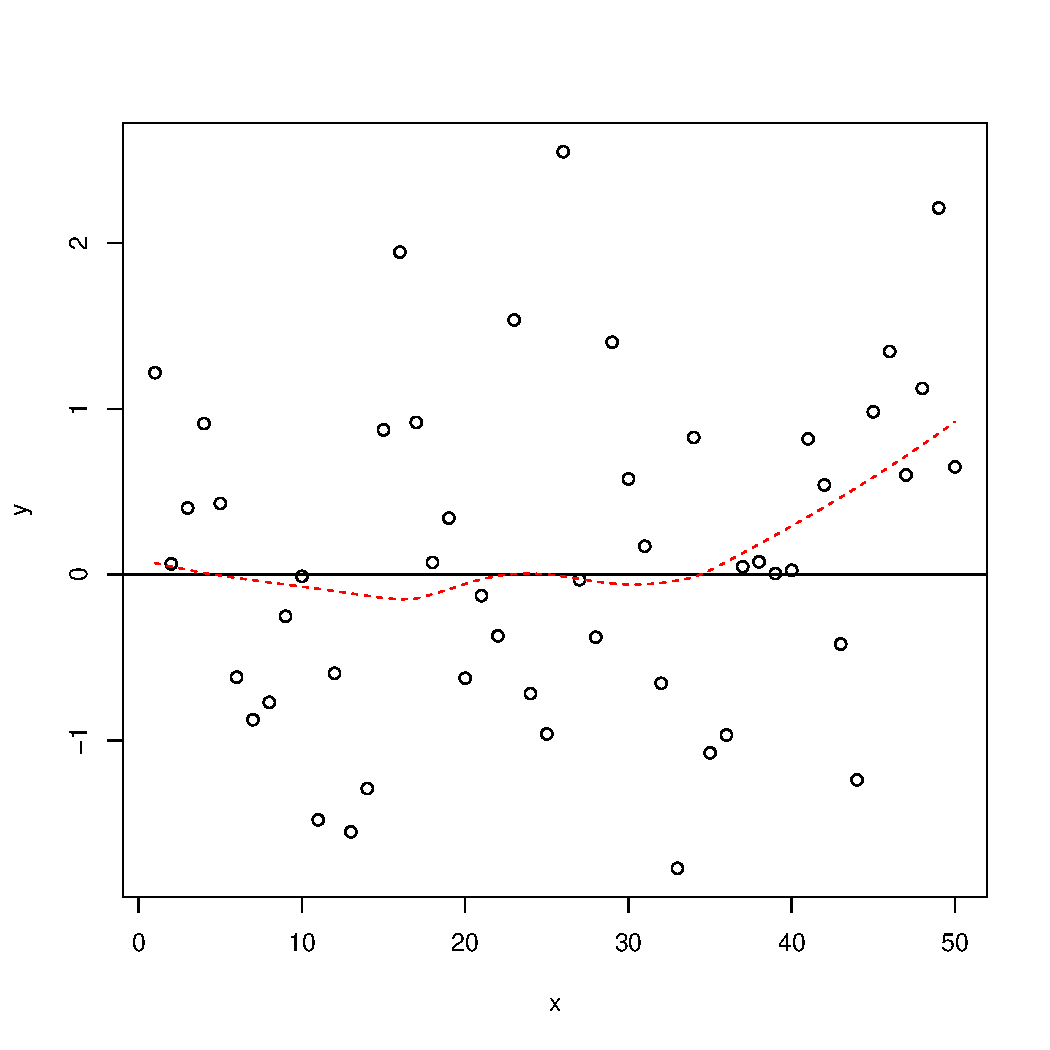
\includegraphics[width=\textwidth]{../15_Diagnostics/convar2.pdf}%filename
                \caption{Linear \label{fig:convar2}}
        \end{subfigure}
        \begin{subfigure}[b]{0.45\textwidth}
                \centering
                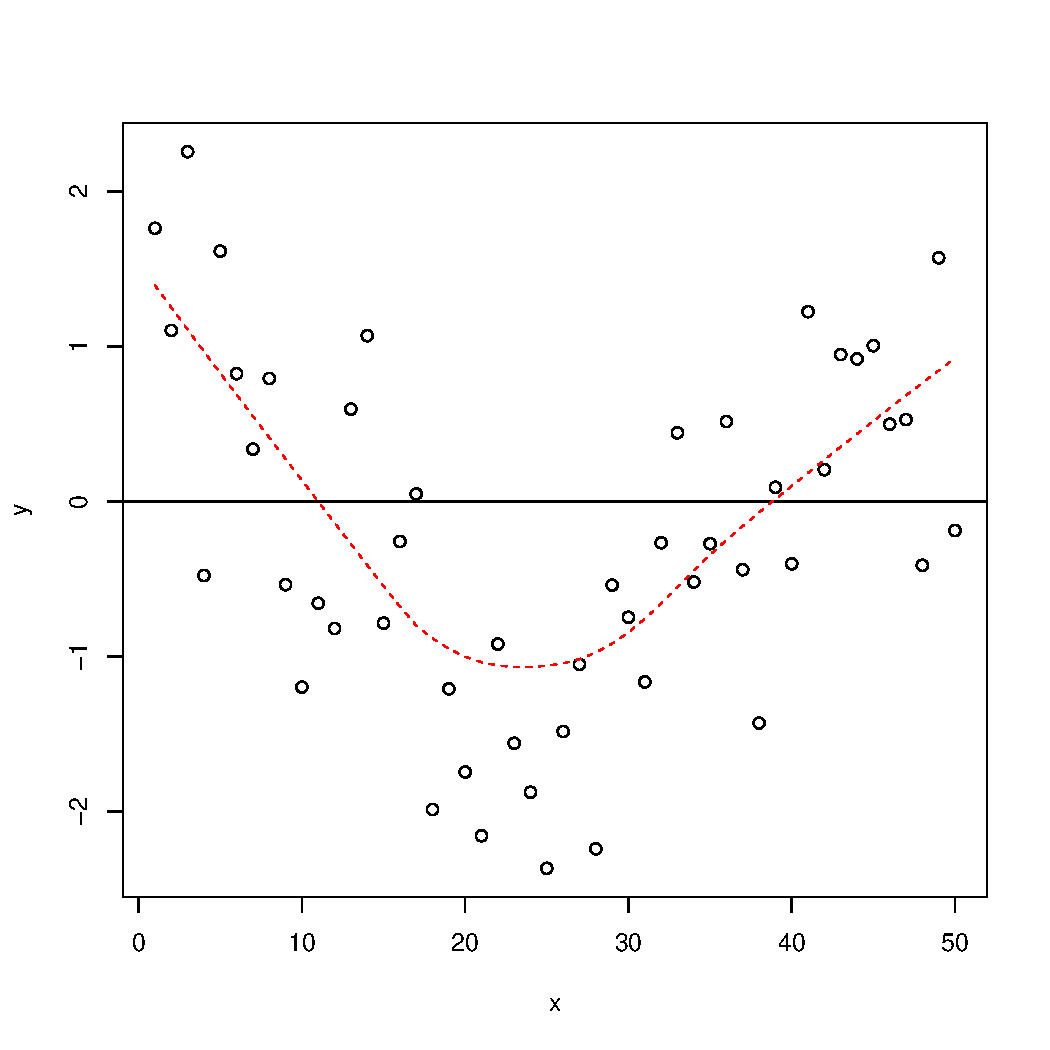
\includegraphics[width=\textwidth]{../15_Diagnostics/nonlin.pdf}
                \caption{Non-Linear \label{fig:nonlin}}
        \end{subfigure}
        \caption{Made Up Residual Examples}
\end{figure} 

Now let's look at the residuals from our example model. We can check the linear nature of the relationship between the DV and the IVs in several ways. First we can plot the residuals by the values of the IVs. We also can add a lowess line to demonstrate the relationship between each of the IVs and the residuals, and add a line at $0$ for comparison. 

\begin{knitrout}
\definecolor{shadecolor}{rgb}{0.969, 0.969, 0.969}\color{fgcolor}\begin{kframe}
\begin{alltt}
\hlstd{ds.small}\hlopt{$}\hlstd{fit.p} \hlkwb{<-} \hlstd{ols1}\hlopt{$}\hlstd{fitted.values}
\hlstd{ds.small} \hlopt
  \hlkwd{melt}\hlstd{(}\hlkwc{measure.vars} \hlstd{=} \hlkwd{c}\hlstd{(}\hlstr{"age"}\hlstd{,} \hlstr{"education"}\hlstd{,} \hlstr{"income"}\hlstd{,} \hlstr{"ideol"}\hlstd{,} \hlstr{"fit.p"}\hlstd{))} \hlopt
  \hlkwd{ggplot}\hlstd{(}\hlkwd{aes}\hlstd{(value, fit.r,} \hlkwc{group} \hlstd{= variable))} \hlopt{+}
  \hlkwd{geom_point}\hlstd{(}\hlkwc{shape} \hlstd{=} \hlnum{1}\hlstd{)} \hlopt{+}
  \hlkwd{geom_smooth}\hlstd{(}\hlkwc{method} \hlstd{= loess)} \hlopt{+}
  \hlkwd{geom_hline}\hlstd{(}\hlkwc{yintercept} \hlstd{=} \hlnum{0}\hlstd{)} \hlopt{+}
  \hlkwd{facet_wrap}\hlstd{(}\hlopt{~} \hlstd{variable,} \hlkwc{scales} \hlstd{=} \hlstr{"free"}\hlstd{)}
\hlkwd{dev.off}\hlstd{()}
\end{alltt}
\end{kframe}
\end{knitrout}
\begin{figure}
        \centering
        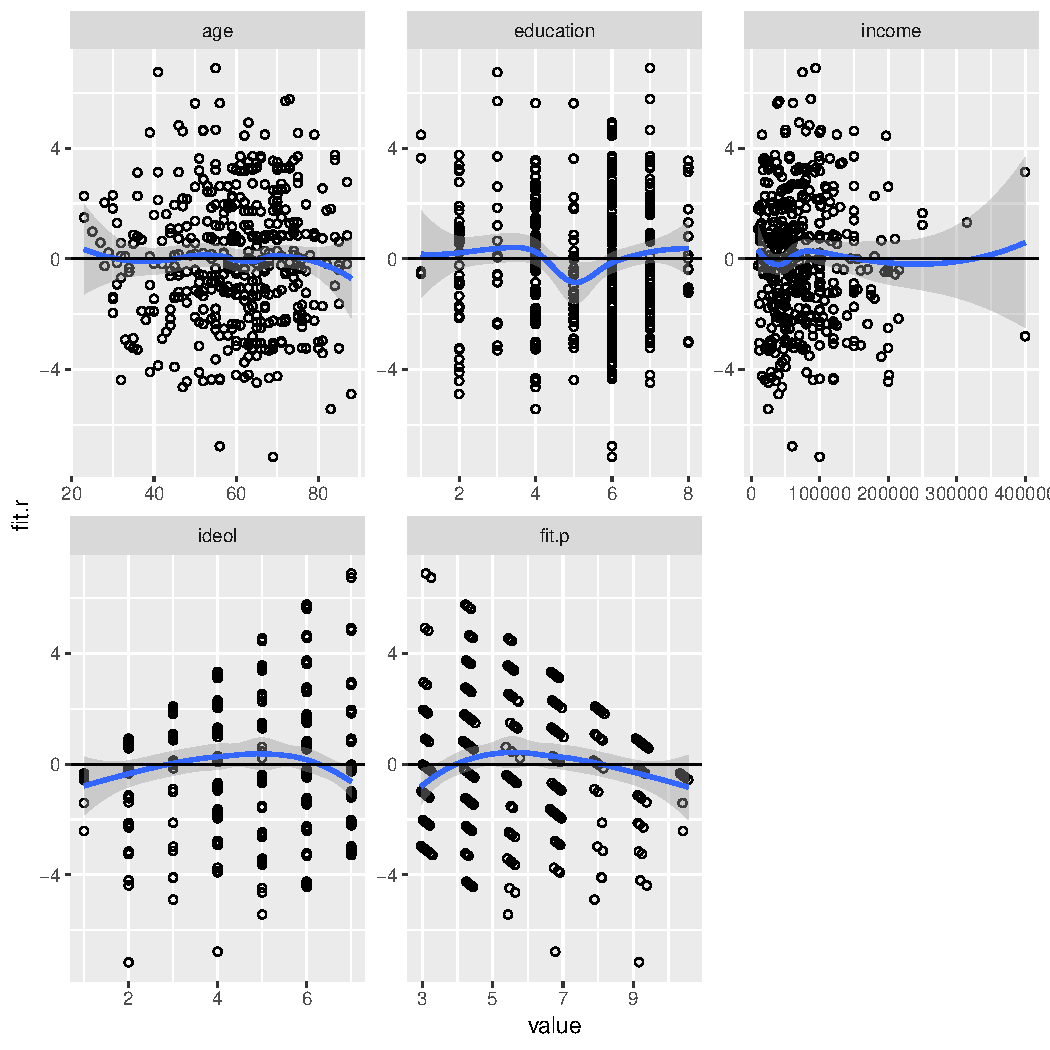
\includegraphics[width=4in]{../15_Diagnostics/multlin.pdf}%filename
        \caption{Checking for Non-Linearity \label{fig:multlin}}
\end{figure}        

\noindent As we can see in Figure \ref{fig:multlin}, the plots of residuals by both income and ideology seem to indicate non-linear relationships. We can check this ``ocular impression" by squaring each term and using the \texttt{anova} function to compare model fit.
\begin{knitrout}
\definecolor{shadecolor}{rgb}{0.969, 0.969, 0.969}\color{fgcolor}\begin{kframe}
\begin{alltt}
\hlstd{ds.small}\hlopt{$}\hlstd{age2} \hlkwb{<-} \hlstd{ds.small}\hlopt{$}\hlstd{age}\hlopt{^}\hlnum{2}
\hlstd{ds.small}\hlopt{$}\hlstd{edu2} \hlkwb{<-} \hlstd{ds.small}\hlopt{$}\hlstd{education}\hlopt{^}\hlnum{2}
\hlstd{ds.small}\hlopt{$}\hlstd{inc2} \hlkwb{<-} \hlstd{ds.small}\hlopt{$}\hlstd{income}\hlopt{^}\hlnum{2}
\hlstd{ds.small}\hlopt{$}\hlstd{ideology2} \hlkwb{<-} \hlstd{ds.small}\hlopt{$}\hlstd{ideol}\hlopt{^}\hlnum{2}
\hlstd{ols2} \hlkwb{<-} \hlkwd{lm}\hlstd{(glbcc_risk} \hlopt{~} \hlstd{age} \hlopt{+} \hlstd{age2} \hlopt{+} \hlstd{education} \hlopt{+} \hlstd{edu2} \hlopt{+} \hlstd{income} \hlopt{+} \hlstd{inc2} \hlopt{+} \hlstd{ideol} \hlopt{+}
    \hlstd{ideology2,} \hlkwc{data} \hlstd{= ds.small)}
\hlkwd{summary}\hlstd{(ols2)}
\end{alltt}
\begin{verbatim}
## 
## Call:
## lm(formula = glbcc_risk ~ age + age2 + education + edu2 + income + 
##     inc2 + ideol + ideology2, data = ds.small)
## 
## Residuals:
##     Min      1Q  Median      3Q     Max 
## -7.1563 -1.5894  0.0389  1.4898  7.3417 
## 
## Coefficients:
##               Estimate Std. Error t value Pr(>|t|)    
## (Intercept)  9.661e+00  1.931e+00   5.004 8.12e-07 ***
## age          2.973e-02  5.735e-02   0.518 0.604385    
## age2        -2.891e-04  5.010e-04  -0.577 0.564175    
## education   -4.814e-01  3.589e-01  -1.341 0.180499    
## edu2         5.132e-02  3.722e-02   1.379 0.168723    
## income       2.853e-06  5.341e-06   0.534 0.593564    
## inc2        -1.131e-11  1.839e-11  -0.615 0.538966    
## ideol       -5.726e-02  3.532e-01  -0.162 0.871279    
## ideology2   -1.327e-01  3.965e-02  -3.347 0.000886 ***
## ---
## Signif. codes:  0 '***' 0.001 '**' 0.01 '*' 0.05 '.' 0.1 ' ' 1
## 
## Residual standard error: 2.33 on 441 degrees of freedom
## Multiple R-squared:  0.4528,	Adjusted R-squared:  0.4429 
## F-statistic: 45.61 on 8 and 441 DF,  p-value: < 2.2e-16
\end{verbatim}
\end{kframe}
\end{knitrout}

\noindent The model output indicates that ideology may have a non-linear relationships with risk perceptions of climate change.     For ideology, only the squared term is significant, indicating that levels of perceived risk of climate change decline at an increasing rate for those on the most conservative end of the scale.  Again, this is consistent with the visual inspection of the relationship between ideology and the residuals in Figure \ref{fig:multlin}.   The question remains whether the introduction of these non-linear (polynomial) terms improves overall model fit.  We can check that with an analysis of variance across the simple model (without polynomial terms) and the models with the squared terms.

\begin{knitrout}
\definecolor{shadecolor}{rgb}{0.969, 0.969, 0.969}\color{fgcolor}\begin{kframe}
\begin{alltt}
\hlkwd{anova}\hlstd{(ols1, ols2)}
\end{alltt}
\begin{verbatim}
## Analysis of Variance Table
## 
## Model 1: glbcc_risk ~ age + education + income + ideol
## Model 2: glbcc_risk ~ age + age2 + education + edu2 + income + inc2 + 
##     ideol + ideology2
##   Res.Df    RSS Df Sum of Sq      F  Pr(>F)  
## 1    445 2464.2                              
## 2    441 2393.2  4    71.059 3.2736 0.01161 *
## ---
## Signif. codes:  0 '***' 0.001 '**' 0.01 '*' 0.05 '.' 0.1 ' ' 1
\end{verbatim}
\end{kframe}
\end{knitrout}


\noindent As we can see, the Anova test indicates that including the squared terms improves model fit, therefore the relationships include nonlinear components. 

A final way to check for non-linearity is Ramsey's Regression Error Specification Test (RESET). This tests the functional form of the model. Similar to our test using squared terms, the RESET tests calculates an $F$ statistic that compares the linear model with a model(s) that raises the IVs to various powers. Specifically, it tests whether there are statistically significant differences in the $R^2$ of each of the models. Similar to a nested $F$ test, it is calculated by: 

\begin{equation}
  \label{eq:reset}
  F = \frac{\frac{R^2_1-R^2_0}{q}}{\frac{1-R^2_1}{n-k_1}}
\end{equation}

\noindent where $R^2_0$ is the $R^2$ of the linear model, $R^2_1$ is the $R^2$ of the polynomial model(s), $q$ is the number of new regressors, and $k_1$ is the number of IVs in the polynomial model(s). The null hypothesis is that the functional relationship between the $X$'s and $Y$ is linear, therefore the coefficients of the second and third powers to the IVs are zero.  If there is a low $p$-value (i.e., if we can reject the null hypothesis), non-linear relationships are suspected.  This test can be run using the \texttt{resettest} function from the \texttt{lmtest} package. Here we are setting the IVs to the second and third powers and we are examining the regressor variables.\footnote{See the \texttt{lmtest} package documentation for more options and information.}   
  
\begin{knitrout}
\definecolor{shadecolor}{rgb}{0.969, 0.969, 0.969}\color{fgcolor}\begin{kframe}
\begin{alltt}
\hlkwd{library}\hlstd{(lmtest)}
\hlkwd{resettest}\hlstd{(ols1,}\hlkwc{power}\hlstd{=}\hlnum{2}\hlopt{:}\hlnum{3}\hlstd{,}\hlkwc{type}\hlstd{=}\hlstr{"regressor"}\hlstd{)}
\end{alltt}
\begin{verbatim}
## 
## 	RESET test
## 
## data:  ols1
## RESET = 2.2752, df1 = 8, df2 = 437, p-value = 0.02157
\end{verbatim}
\end{kframe}
\end{knitrout}

\noindent Again, the test provides evidence that we have a non-linear relationship. 

What should we do when we identify a nonlinear relationship between our $Y$ and $X$s ?  The first step is to look closely at the bi-variate plots, to try to discern the correct functional form for each $X$ regressor. If the relationship looks curvilinear, try a polynomial regression in which you include both $X$ and $X^2$ for the relevant IVs. It may also be the case that a skewed DV or IV is causing the problem. This is not unusual when, for example, the income variable plays an important role in the model, and the distribution of income is skewed upward. In such a case, you can try transforming the skewed variable, using an appropriate log form.

It is possible that variable transformations won't suffice, however. In that case, you may have no other option by to try non-linear forms of regression. These non-OLS kinds of models typically use maximal likelihood functions (see the next chapter) to fit the model to the data. But  that takes us considerably beyond the focus of this book.

\subsection{Non-Constant Variance, or Heteroscedasticity}

Recall that OLS requires constant variance because the even spread of residuals is assumed for both $F$ and $t$ tests. To examine constant variance, we can produce (read as ``make up") a baseline plot to demonstrate what constant variance in the residuals ``should" look like. 

As we can see in Figure \ref{fig:convar15}, the residuals are spread evenly and in a seemingly random fashion, much like the ``sneeze plot" discussed in Chapter 10.  This is the ideal pattern, indicating that the residuals do not vary systematically over the range of the predicted value for $X$. The residuals are homoscedastistic, and thus provide the appropriate basis for the $F$ and $t$ tests needed for evaluating your hypotheses.

We can also present a clearly heteroscedastistic residual term. In this case the residuals do vary systematically over the range of $X$, indicating that the precision of the estimates of $Y$ will vary considerably over the range of predicted values. Note the distinctive fan shape in Figure \ref{fig:hetero15}, indicating that predictions of $Y$ lose precision as the value of $X$ increases. 



\begin{figure}
        \centering
        \begin{subfigure}[b]{0.45\textwidth}
                \centering
                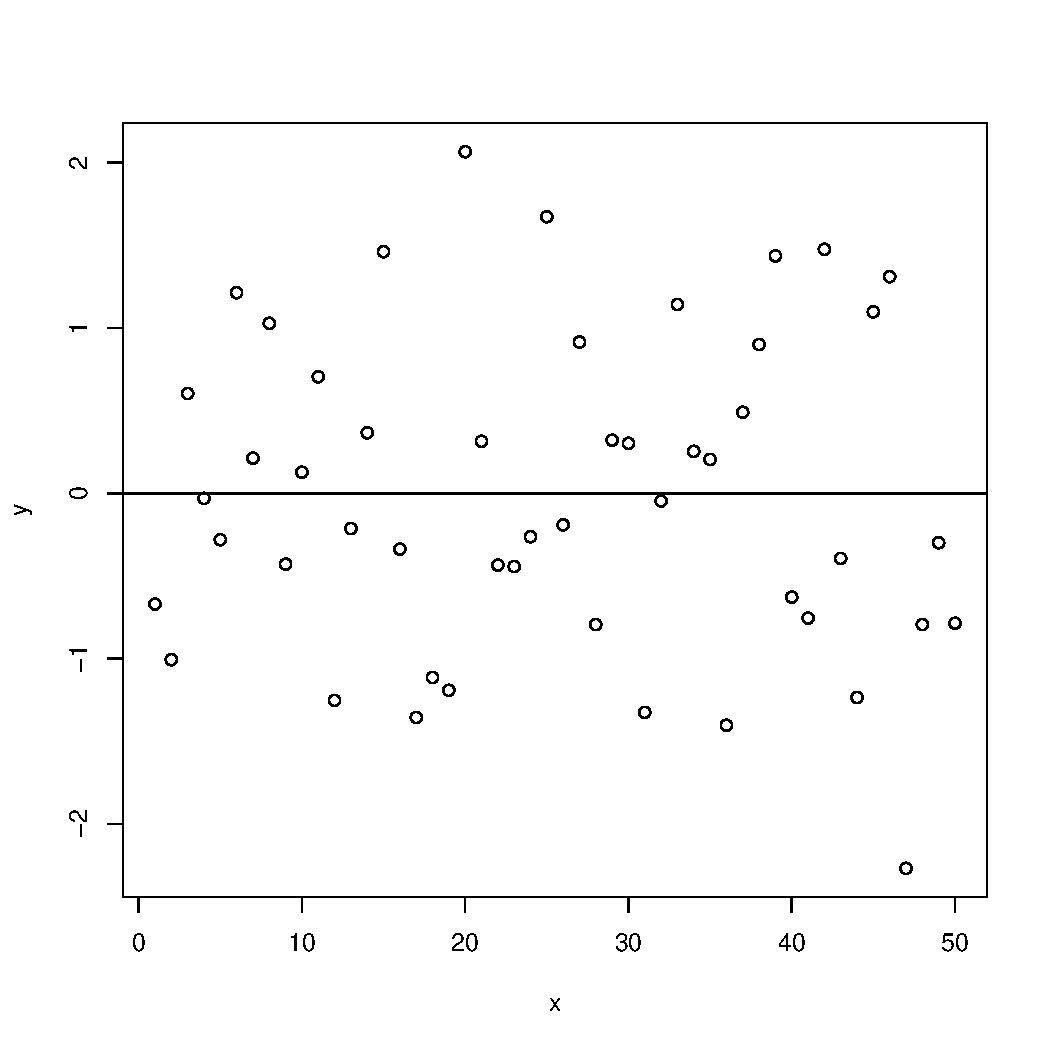
\includegraphics[width=\textwidth]{../15_Diagnostics/convar.pdf}%filename
                \caption{Constant Variance \label{fig:convar15}}
        \end{subfigure}
        \begin{subfigure}[b]{0.45\textwidth}
                \centering
                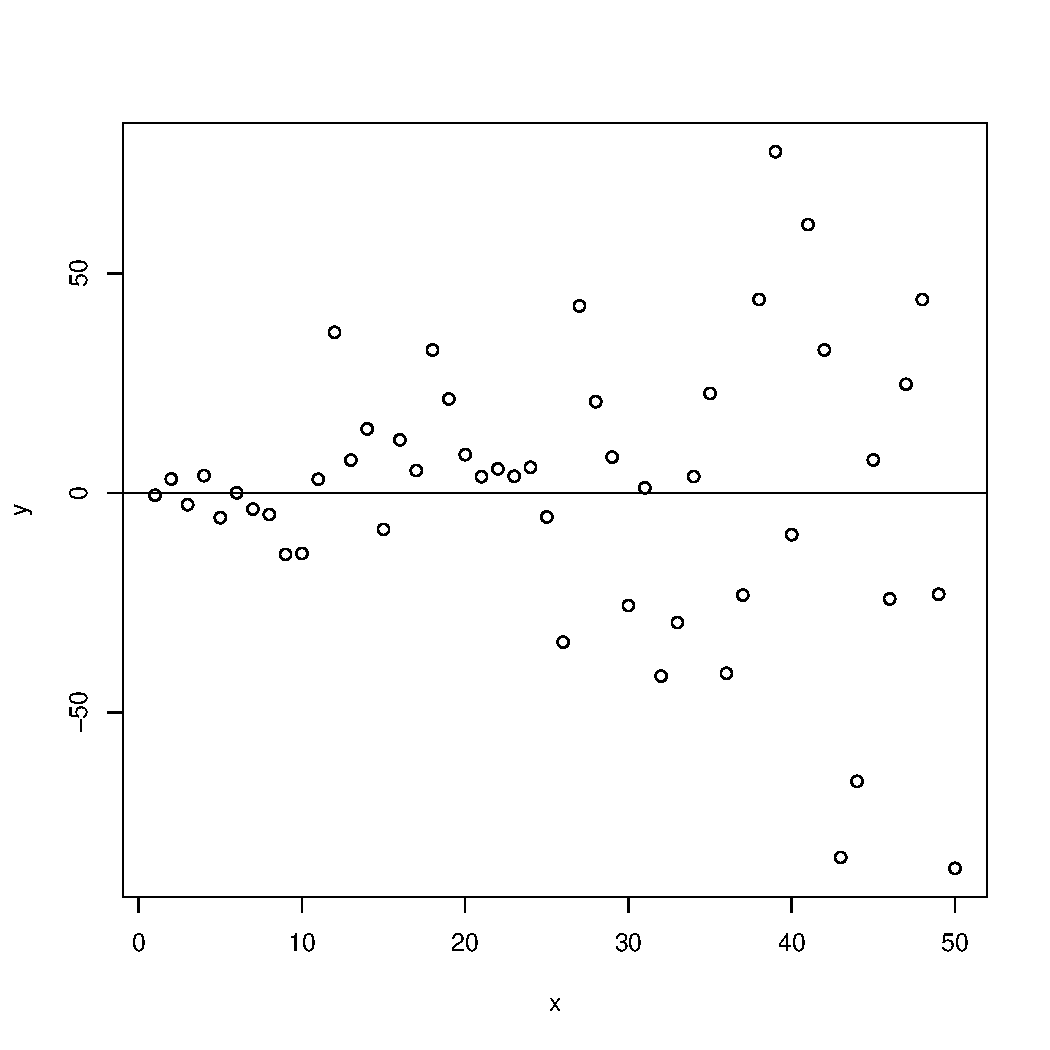
\includegraphics[width=\textwidth]{../15_Diagnostics/heterovar.pdf}%filename
                \caption{Heteroscedasticity \label{fig:hetero15}}
        \end{subfigure}
        \caption{Made Up Residual Examples}
\end{figure}  

The first step in determining whether we have constant variance is to plot the the residuals by the fitted values for $Y$, as follows:\footnote{Note that we jitter the points to make them easier to see.}

\begin{knitrout}
\definecolor{shadecolor}{rgb}{0.969, 0.969, 0.969}\color{fgcolor}\begin{kframe}
\begin{alltt}
\hlstd{ds.small}\hlopt{$}\hlstd{fit.r} \hlkwb{<-} \hlstd{ols1}\hlopt{$}\hlstd{residuals}
\hlstd{ds.small}\hlopt{$}\hlstd{fit.p} \hlkwb{<-} \hlstd{ols1}\hlopt{$}\hlstd{fitted.values}
\end{alltt}
\end{kframe}
\end{knitrout}

\begin{figure}
        \centering
        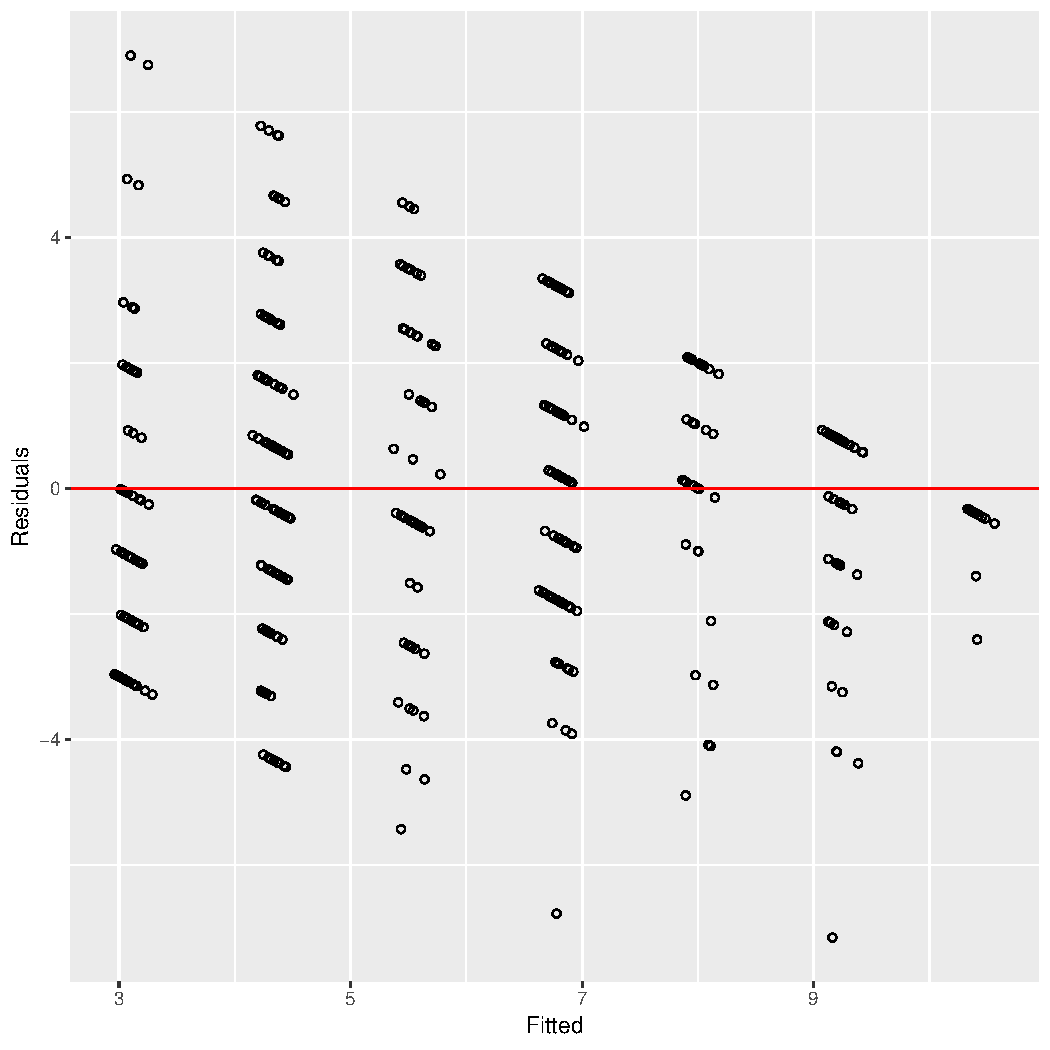
\includegraphics[width=4in]{../15_Diagnostics/multregres.pdf}%filename
        \caption{Multiple Regression Residuals and Fitted Values \label{fig:multregres}}
\end{figure}

\noindent Based on the pattern evident in Figure \ref{fig:multregres}, the residuals
appear to show heteroscedasticity. We can test for non-constant error using the Breusch-Pagan (aka Cook-Weisberg) test. This tests the null hypothesis that the error variance is constant, therefore a small p value would indicate that we have heteroscedasticity. In R we can use the ncvTest function from the car package.

\begin{knitrout}
\definecolor{shadecolor}{rgb}{0.969, 0.969, 0.969}\color{fgcolor}\begin{kframe}
\begin{alltt}
\hlkwd{library}\hlstd{(car)}
\hlkwd{ncvTest}\hlstd{(ols1)}
\end{alltt}
\begin{verbatim}
## Non-constant Variance Score Test 
## Variance formula: ~ fitted.values 
## Chisquare = 12.70938    Df = 1     p = 0.0003638269
\end{verbatim}
\end{kframe}
\end{knitrout}
\noindent The non-constant variance test provides confirmation that the residuals from our model are heteroscedastistic.

What are the implications? Our $t$-tests for the estimated partial regression  coefficients assumed constant variance. With the evidence of heteroscedasticity, we conclude that these tests are unreliable (the precision of our estimates will be greater in some ranges of $X$ than others). 

They are several steps that can be considered when confronted by heteroscedasticity in the residuals. First, we can consider whether we need to re-specify the model, possibly because we have some omitted variables. If model re-specification does not correct the problem, we can use non-OLS regression techniques that include robust estimated  standard errors.  Robust standard errors are appropriate when error variance is unknown. Robust standard errors do not change the estimate of $B$, but adjust the estimated standard error of each coefficient, $SE(B)$, thus giving more accurate $p$ values. In this example, we draw on White's (1980)\footnote{H White,  1980.  ``A Heteroskedasticity-consistent covariance matrix estimator and a direct test for heteroskedasticity." \underline{Econometrica} 48: 817-838.} method to calculate robust standard errors.  

White uses a \textbf{heteroskedasticity consistent covariance matrix} (hccm) to calculate standard errors when the error term has non-constant variance. Under the OLS assumption of constant error variance, the covariance matrix of $b$ is:
\begin{equation*}
  V(b) = (X'X)^{-1} X'V(y)X(X'X)^{-1}
\end{equation*}
\noindent where $V(y)=\sigma^{2}_{e}I_n$, therefore,
$V(b)=\sigma^{2}_{e}(X'X)^{-1}$. If the error terms have distinct
variances, a consistent estimator constrains $\Sigma$ to a diagonal
matrix of the squared residuals,
$\Sigma=\text{diag}(\sigma^2_1,\ldots,\sigma^2_n)$ where $\sigma^2_i$
is estimated by $e^2_i$. Therefore the hccm estimator is expressed as:  
\begin{equation*}
 V_{hccm}(b) = (X'X)^{-1} X'\text{diag}(e^2_i,\ldots,e^2_n) X(X'X)^{-1} 
\end{equation*}

We can use the \texttt{hccm} function from the \texttt{car} package to calculate the robust standard errors for our regression model, predicting perceived environmental risk ($Y$) with political ideology, age, education and income as the $X$ variables. 
\begin{knitrout}
\definecolor{shadecolor}{rgb}{0.969, 0.969, 0.969}\color{fgcolor}\begin{kframe}
\begin{alltt}
\hlkwd{library}\hlstd{(car)}
\hlkwd{hccm}\hlstd{(ols1)} \hlopt \hlkwd{diag}\hlstd{()} \hlopt \hlkwd{sqrt}\hlstd{()}
\end{alltt}
\begin{verbatim}
##  (Intercept)          age    education       income        ideol 
## 6.687787e-01 8.030366e-03 6.982449e-02 2.320899e-06 6.003903e-02
\end{verbatim}
\end{kframe}
\end{knitrout}

Using the \texttt{hccm} function we can create a function in \texttt{R} that will calculate the robust standard errors and the subsequent $t$-values and $p$-values. 
\begin{knitrout}
\definecolor{shadecolor}{rgb}{0.969, 0.969, 0.969}\color{fgcolor}\begin{kframe}
\begin{alltt}
\hlkwd{library}\hlstd{(car)}
\hlstd{robust.se} \hlkwb{<-} \hlkwa{function}\hlstd{(}\hlkwc{model}\hlstd{) \{}
  \hlstd{s} \hlkwb{<-} \hlkwd{summary}\hlstd{(model)}
  \hlstd{wse} \hlkwb{<-} \hlkwd{sqrt}\hlstd{(}\hlkwd{diag}\hlstd{(}\hlkwd{hccm}\hlstd{(ols1)))}
  \hlstd{t} \hlkwb{<-} \hlstd{model}\hlopt{$}\hlstd{coefficients}\hlopt{/}\hlstd{wse}
  \hlstd{p} \hlkwb{<-} \hlnum{2}\hlopt{*}\hlkwd{pnorm}\hlstd{(}\hlopt{-}\hlkwd{abs}\hlstd{(t))}
  \hlstd{results} \hlkwb{<-} \hlkwd{cbind}\hlstd{(model}\hlopt{$}\hlstd{coefficients, wse, t, p)}
  \hlkwd{dimnames}\hlstd{(results)} \hlkwb{<-} \hlkwd{dimnames}\hlstd{(s}\hlopt{$}\hlstd{coefficients)}
  \hlstd{results}
\hlstd{\}}
\end{alltt}
\end{kframe}
\end{knitrout}

We can then compare our results with the original simple regression model results. 
\begin{knitrout}
\definecolor{shadecolor}{rgb}{0.969, 0.969, 0.969}\color{fgcolor}\begin{kframe}
\begin{alltt}
\hlkwd{summary}\hlstd{(ols1)}
\end{alltt}
\begin{verbatim}
## 
## Call:
## lm(formula = glbcc_risk ~ age + education + income + ideol, data = ds.small)
## 
## Residuals:
##     Min      1Q  Median      3Q     Max 
## -7.1617 -1.7131 -0.0584  1.7216  6.8981 
## 
## Coefficients:
##               Estimate Std. Error t value Pr(>|t|)    
## (Intercept)  1.208e+01  7.247e-01  16.676   <2e-16 ***
## age         -5.559e-03  8.407e-03  -0.661    0.509    
## education   -1.861e-02  6.979e-02  -0.267    0.790    
## income       1.923e-07  2.227e-06   0.086    0.931    
## ideol       -1.224e+00  6.630e-02 -18.454   <2e-16 ***
## ---
## Signif. codes:  0 '***' 0.001 '**' 0.01 '*' 0.05 '.' 0.1 ' ' 1
## 
## Residual standard error: 2.353 on 445 degrees of freedom
## Multiple R-squared:  0.4365,	Adjusted R-squared:  0.4315 
## F-statistic: 86.19 on 4 and 445 DF,  p-value: < 2.2e-16
\end{verbatim}
\begin{alltt}
\hlkwd{robust.se}\hlstd{(ols1)}
\end{alltt}
\begin{verbatim}
##                  Estimate   Std. Error      t value     Pr(>|t|)
## (Intercept)  1.208483e+01 6.687787e-01  18.06999168 5.492199e-73
## age         -5.558580e-03 8.030366e-03  -0.69219509 4.888148e-01
## education   -1.861467e-02 6.982449e-02  -0.26659225 7.897831e-01
## income       1.922905e-07 2.320899e-06   0.08285175 9.339694e-01
## ideol       -1.223565e+00 6.003903e-02 -20.37948994 2.542911e-92
\end{verbatim}
\end{kframe}
\end{knitrout}
\noindent As we see the estimated $B$'s remain the same, but the estimated standard errors, $t$-values and $p$-values are adjusted to reflect the robust estimation. Despite these adjustments, the results of the hypothesis test remain unchanged.

It is important to note that, while robust estimators can help atone for heteroscedasticity in your models, their use \texttt{should not} be seen as an alternative to careful model construction. The first step should always be to evaluate your model specification and functional form (e.g., the use of polynomials, inclusion of relevant variables), as well as possible measurement error, before resorting to robust estimation.

\subsection{Independence of $E$} 

As noted above, we cannot test for the assumption that the error term $E$ is independent of the $X$'s.  However we can test to see whether the error terms, $E_i$, are correlated with each other. One of the assumptions of OLS is that   $E(\epsilon_i) \neq E(\epsilon_j)$ for $i \neq j$. When there is a relationship between the residuals, this is referred to as serial correlation or \textbf{autocorrelation}. Autocorrelation is most likely to occur with time-series data, however it can occur with cross-sectional data as well. To test for autocorrelation we use the Durbin-Watson, $d$, test statistic. The $d$ statistic is expressed as:

\begin{equation}
  \label{eq:dw}
  d = \frac{\sum_{i=2}^{n} (E_i-E_{i-1})^{2}}{\sum_{i=1}^{n} E^{2}_i}
\end{equation}

The $d$ statistics ranges from $0$ to $4$; $0 \leq d \leq 4$. A  $0$ indicates perfect positive correction, $4$ indicates perfect negative correlation, and a $2$ indicates no autocorrelation. Therefore, we look for values of $d$ that are close to $2$.  

We can use the \texttt{dwtest} function in the \texttt{lmtest} package to test the null hypothesis that autocorrelation is $0$, meaning that we don't have autocorrelation. 

\begin{knitrout}
\definecolor{shadecolor}{rgb}{0.969, 0.969, 0.969}\color{fgcolor}\begin{kframe}
\begin{alltt}
\hlkwd{library}\hlstd{(lmtest)}
\hlkwd{dwtest}\hlstd{(ols1)}
\end{alltt}
\begin{verbatim}
## 
## 	Durbin-Watson test
## 
## data:  ols1
## DW = 1.9008, p-value = 0.1441
## alternative hypothesis: true autocorrelation is greater than 0
\end{verbatim}
\end{kframe}
\end{knitrout}
\noindent Generally, a Durbin-Watson result between 1.5 and 2.5 indicates, that any autocorrelation in the data will not have a discernible effect on your estimates.  The test for our example model indicates that we do not have an autocorrelation problem with this model. If we did find autocorrelation, we would need to respecify our model to account for (or estimate) the relationships among the error terms. In time series analysis, where observations are taken sequentially over time, we would typically include a ``lag" term (in which the value of $Y$ in period $t$ is predicted by the value of $Y$ in period $t-1$). This is a typical $AR1$ model, which would be discussed in a time-series analysis course. The entangled residuals  can, of course, be much more complex, and require more specialized models (e.g.,  ARIMA or vector-autoregression models). These approaches are beyond the  scope of this text.

\subsection{Normality of the Residuals} 

This is a critical assumption for OLS because (along with homoscedasticity) it is required for  hypothesis tests and confidence interval estimation. It is particularly sensitive with small samples. Note that non-normality will increase sample-to-sample variation in model estimates. 

To examine normality of the residuals we first plot the residuals and then run what is known as the Shapiro-Wilk normality test. Here we run the test on our example model, and plot the residuals.

\begin{knitrout}
\definecolor{shadecolor}{rgb}{0.969, 0.969, 0.969}\color{fgcolor}\begin{kframe}
\begin{alltt}
\hlkwd{ggplot}\hlstd{(ds.small,} \hlkwd{aes}\hlstd{(fit.r))} \hlopt{+}
  \hlkwd{geom_histogram}\hlstd{(}\hlkwc{bins} \hlstd{=} \hlnum{10}\hlstd{,} \hlkwc{color} \hlstd{=} \hlstr{"black"}\hlstd{,} \hlkwc{fill} \hlstd{=} \hlstr{"white"}\hlstd{)}
\end{alltt}
\end{kframe}
\end{knitrout}

\begin{knitrout}
\definecolor{shadecolor}{rgb}{0.969, 0.969, 0.969}\color{fgcolor}\begin{kframe}
\begin{alltt}
\hlkwd{ggplot}\hlstd{(ds.small,} \hlkwd{aes}\hlstd{(fit.r))} \hlopt{+}
  \hlkwd{geom_density}\hlstd{()} \hlopt{+}
  \hlkwd{stat_function}\hlstd{(}\hlkwc{fun} \hlstd{= dnorm,} \hlkwc{args} \hlstd{=} \hlkwd{list}\hlstd{(}\hlkwc{mean} \hlstd{=} \hlkwd{mean}\hlstd{(ds.small}\hlopt{$}\hlstd{fit.r),}
                                         \hlkwc{sd} \hlstd{=} \hlkwd{sd}\hlstd{(ds.small}\hlopt{$}\hlstd{fit.r)),}
                \hlkwc{color} \hlstd{=} \hlstr{"dodgerblue"}\hlstd{,} \hlkwc{size} \hlstd{=} \hlnum{2}\hlstd{,} \hlkwc{alpha} \hlstd{=} \hlnum{.5}\hlstd{)}
\hlkwd{dev.off}\hlstd{()}
\end{alltt}
\end{kframe}
\end{knitrout}
 
\begin{knitrout}
\definecolor{shadecolor}{rgb}{0.969, 0.969, 0.969}\color{fgcolor}\begin{kframe}
\begin{alltt}
\hlkwd{ggplot}\hlstd{(ds.small,} \hlkwd{aes}\hlstd{(}\hlstr{""}\hlstd{, fit.r))} \hlopt{+}
  \hlkwd{geom_boxplot}\hlstd{()}
\end{alltt}
\end{kframe}
\end{knitrout}

\begin{knitrout}
\definecolor{shadecolor}{rgb}{0.969, 0.969, 0.969}\color{fgcolor}\begin{kframe}
\begin{alltt}
\hlkwd{ggplot}\hlstd{(ds.small,} \hlkwd{aes}\hlstd{(}\hlkwc{sample} \hlstd{= fit.r))} \hlopt{+}
  \hlkwd{stat_qq}\hlstd{(}\hlkwc{shape} \hlstd{=} \hlnum{1}\hlstd{)} \hlopt{+}
  \hlkwd{stat_qq_line}\hlstd{(}\hlkwc{size} \hlstd{=} \hlnum{1.5}\hlstd{,} \hlkwc{alpha} \hlstd{=} \hlnum{.5}\hlstd{)}
\hlkwd{dev.off}\hlstd{()}
\end{alltt}
\end{kframe}
\end{knitrout}

\begin{figure}
        \centering
        \begin{subfigure}[b]{0.4\textwidth}
                \centering
                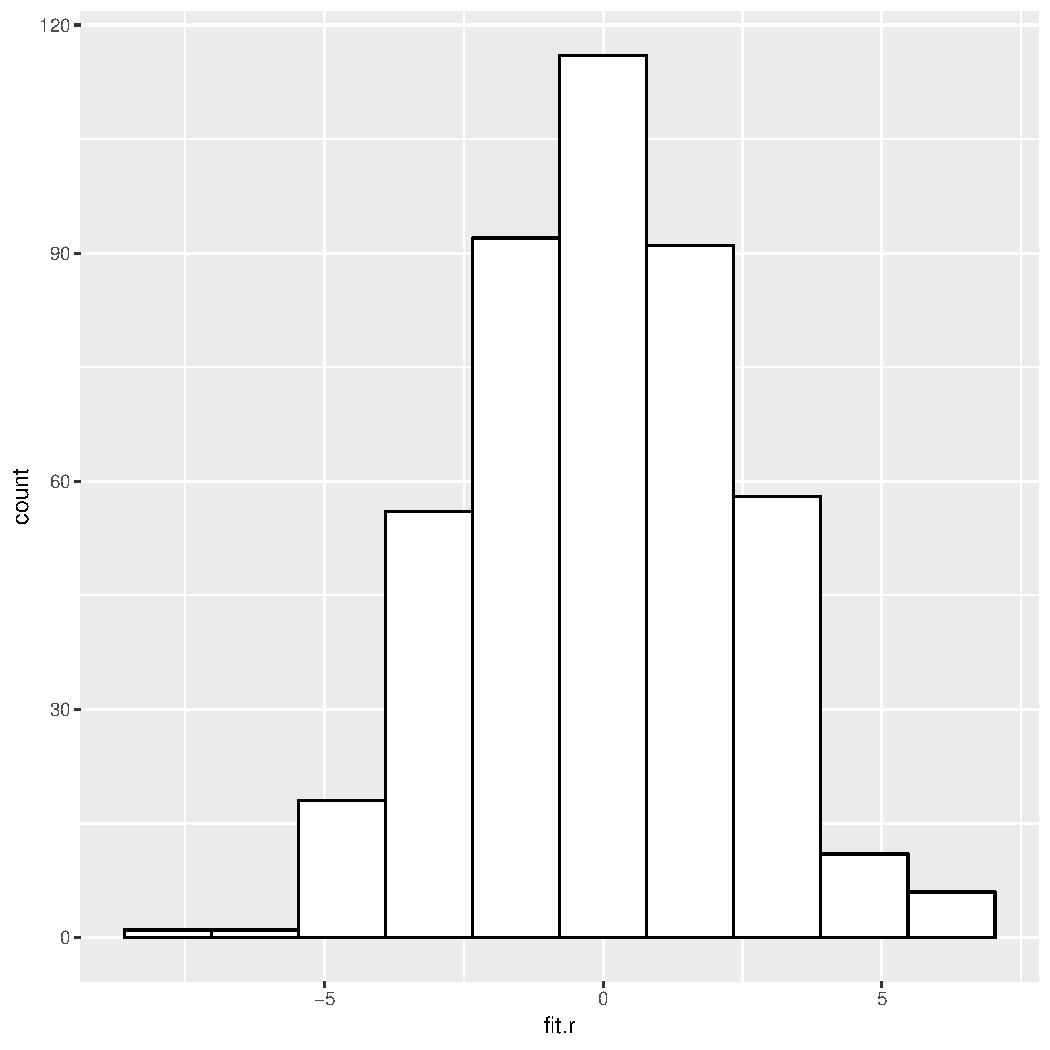
\includegraphics[width=\textwidth]{../15_Diagnostics/multresidhist2.pdf} %filename
                \caption{Histogram \label{fig:multresidhist2}}
        \end{subfigure}
        \begin{subfigure}[b]{0.4\textwidth}
                \centering
                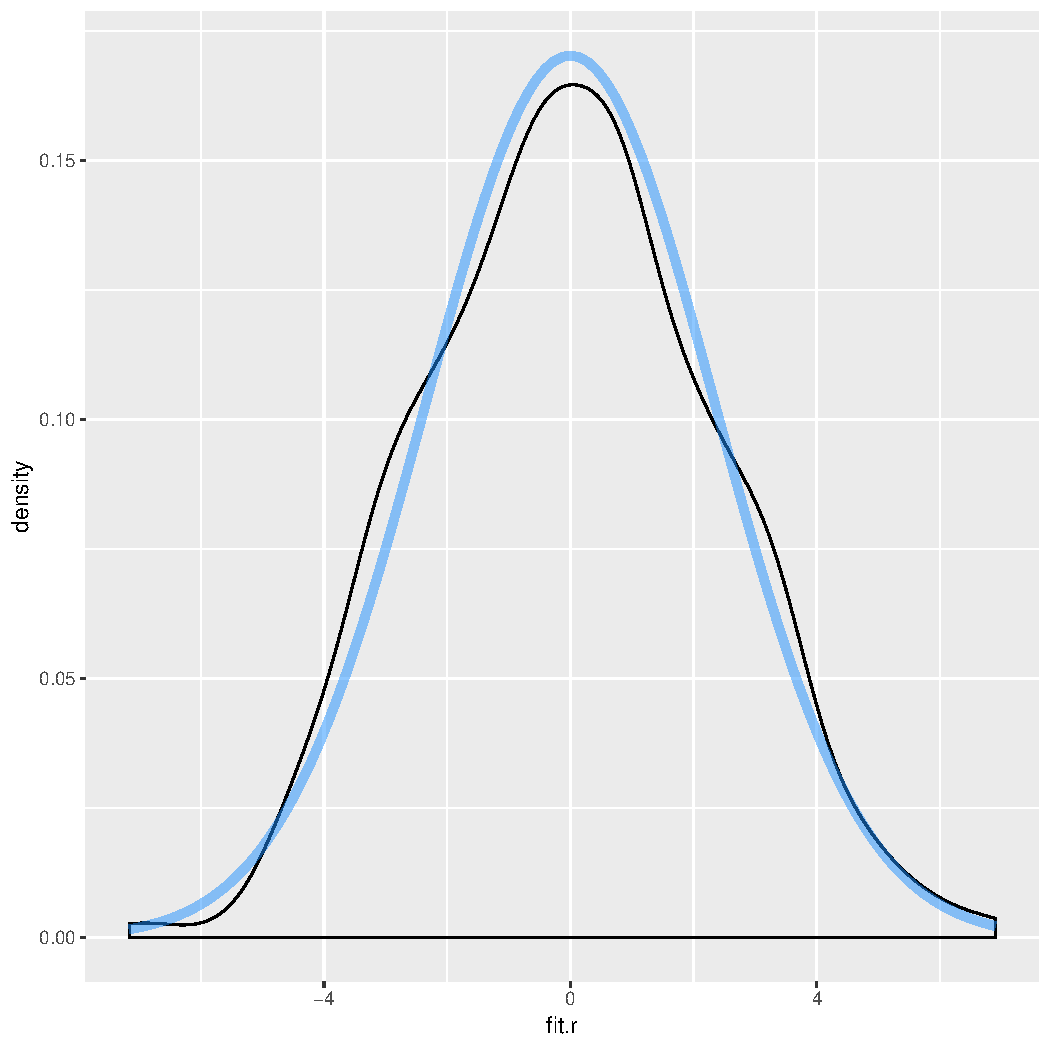
\includegraphics[width=\textwidth]{../15_Diagnostics/multresidden2.pdf} %filename
                \caption{Density \label{fig:multresidden2}}
        \end{subfigure}
        \begin{subfigure}[b]{0.4\textwidth}
                \centering
                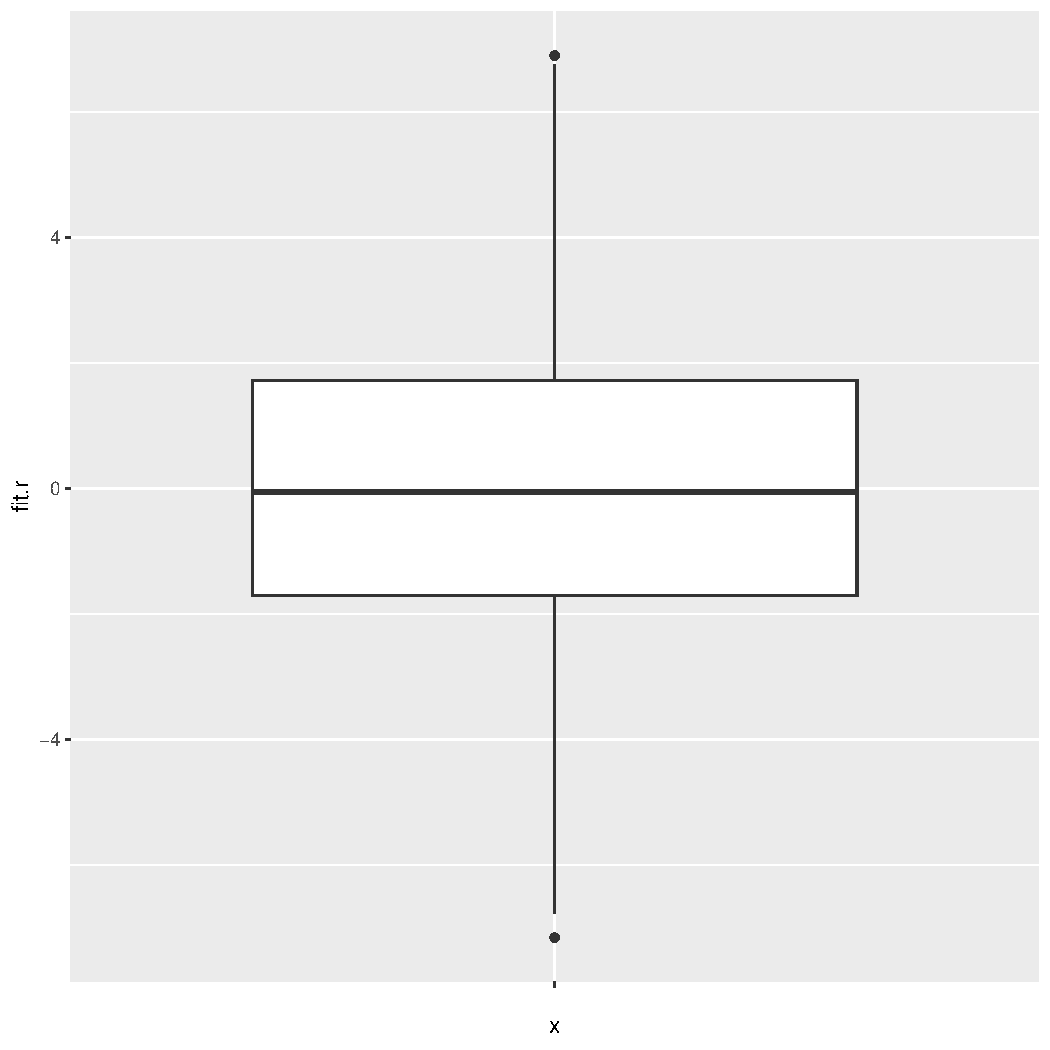
\includegraphics[width=\textwidth]{../15_Diagnostics/multresidbox.pdf} %filename
                \caption{Boxplot \label{fig:multresidbox}}
        \end{subfigure}
        \begin{subfigure}[b]{0.4\textwidth}
                \centering
                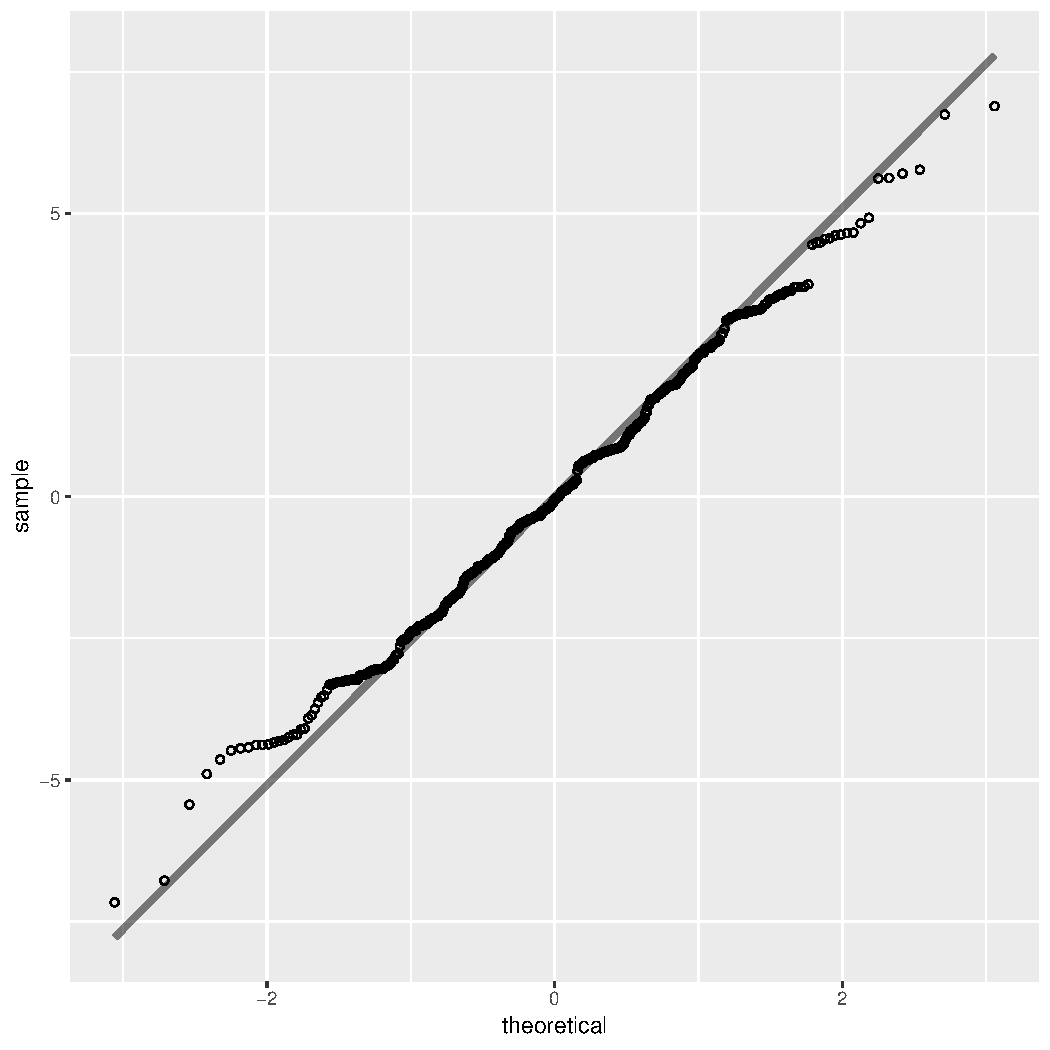
\includegraphics[width=\textwidth]{../15_Diagnostics/multresidqq.pdf} %filename
                \caption{QQ Plot \label{fig:multresidqq}}
        \end{subfigure}
        \caption{Multiple Regression Residuals}
\end{figure}


It appears from the graphs, on the basis of an ``ocular test", that the residuals are potentially normally distributed.  Therefore, to perform a statistical test for non-normality, we use the Shapiro-Wilk, $W$, test statistic. $W$ is expressed as: 
\begin{equation}
  \label{eq:sw}
  W = \frac{(\sum_{i=1}^{n} a_i x_{(i)})^{2}}{\sum_{i=1}^{n} (x_i-\bar{x})^{2}}
\end{equation}
\noindent where $x_{(i)}$ are the ordered sample values and $a_i$ are constants generated from the means, variances, and covariances of the order statistics from a normal distribution. 
The Shapiro-Wilk tests the null hypothesis that the residuals are normally distributed. To perform this test in \texttt{R}, use the \texttt{shapiro.test} function.   
\begin{knitrout}
\definecolor{shadecolor}{rgb}{0.969, 0.969, 0.969}\color{fgcolor}\begin{kframe}
\begin{alltt}
\hlkwd{shapiro.test}\hlstd{(ols1}\hlopt{$}\hlstd{residuals)}
\end{alltt}
\begin{verbatim}
## 
## 	Shapiro-Wilk normality test
## 
## data:  ols1$residuals
## W = 0.99566, p-value = 0.2485
\end{verbatim}
\end{kframe}
\end{knitrout}
\noindent Since we have a relatively large $p$ value we fail to reject the null hypothesis of normally distributed errors.  Our residuals are, accoridng to our visual examination and this test, normally distributed. 

To adjust for non-normal errors we can use robust estimators, as discussed earlier with respect to heteroscedasticity. Robust estimators correct for non-normality, but produce estimated standard errors of the partial regression coefficients that tend to be larger, and hence produce less model precision. Other possible steps, where warranted, include transformation of variables that may have non-linear relationships with $Y$. Typically this involves taking log transformations of the suspect variables. 

\subsection{Outliers, Leverage, and Influence} 

Apart from the distributional behavior of residuals, it is also important to examine the residuals for ``unusual" observations. Unusual observations in the data may be cases of mis-coding (e.g., $-99$), mis-measurement, or perhaps special cases that require different kinds of treatment in the model. All of these may appear as unusual cases that are observed in your diagnostic analysis. The unusual cases that we should be most concerned about are regression outliers, that are potentially influential and that are suspect because of their differences from other cases.

Why should we worry about outliers? Recall that OLS minimizes the sum of the squared residuals for a model. Unusual cases -- which by definition will have large outliers -- have the potential to substantially influence our estimates of $B$ because their already large residuals are squared. A large outlier can thus result in OLS estimates that change the model intercept and slope.

There are several steps that can help identify outliers and their effects on your model. The first -- and most obvious -- is to examine the range of values in your $Y$ and $X$ variables. Do they fall within the appropriate ranges?

This step -- too often omitted even by experienced analysts -- can help you avoid often agonizing mis-steps that result from inclusion of miscoded data or missing values (e.g., ``-99") that need to be recoded before running your model. If you fail to identify these problems, they will show up in your residual analysis as outliers. But it is much easier to catch the problem \texttt{before} you run your model.

But sometimes we find outliers for reasons other than mis-codes, and identification requires careful examination of your residuals.  First we discuss how to find outliers -- unusual values of $Y$ -- and leverage -- unusual values of $X$ -- since they are closely related.  

\subsubsection{Outliers}

A regression outlier is an observation that has an unusual value on the dependent variable $Y$, conditioned on the values of the independent variables, $X$. Note that an outlier can have a large residual value, but not necessarily affect the estimated slope or intercept. Below we examine a few ways to identify potential outliers, and their effects on our estimated slope coefficients.   

Using the regression example, we first plot the residuals to look for any possible outliers. In this plot we are plotting the raw residuals for each of the $500$ observations. This is shown in Figure \ref{fig:siminresid}.  

% residual plot 
\begin{knitrout}
\definecolor{shadecolor}{rgb}{0.969, 0.969, 0.969}\color{fgcolor}\begin{kframe}
\begin{alltt}
\hlkwd{ggplot}\hlstd{(ds.small,} \hlkwd{aes}\hlstd{(}\hlkwd{row.names}\hlstd{(ds.small), fit.r))} \hlopt{+}
  \hlkwd{geom_point}\hlstd{(}\hlkwc{shape} \hlstd{=} \hlnum{1}\hlstd{)} \hlopt{+}
  \hlkwd{geom_hline}\hlstd{(}\hlkwc{yintercept} \hlstd{=} \hlnum{0}\hlstd{,} \hlkwc{color} \hlstd{=} \hlstr{"red"}\hlstd{)}
\hlkwd{dev.off}\hlstd{()}
\end{alltt}
\end{kframe}
\end{knitrout}

\begin{figure}
        \centering
       %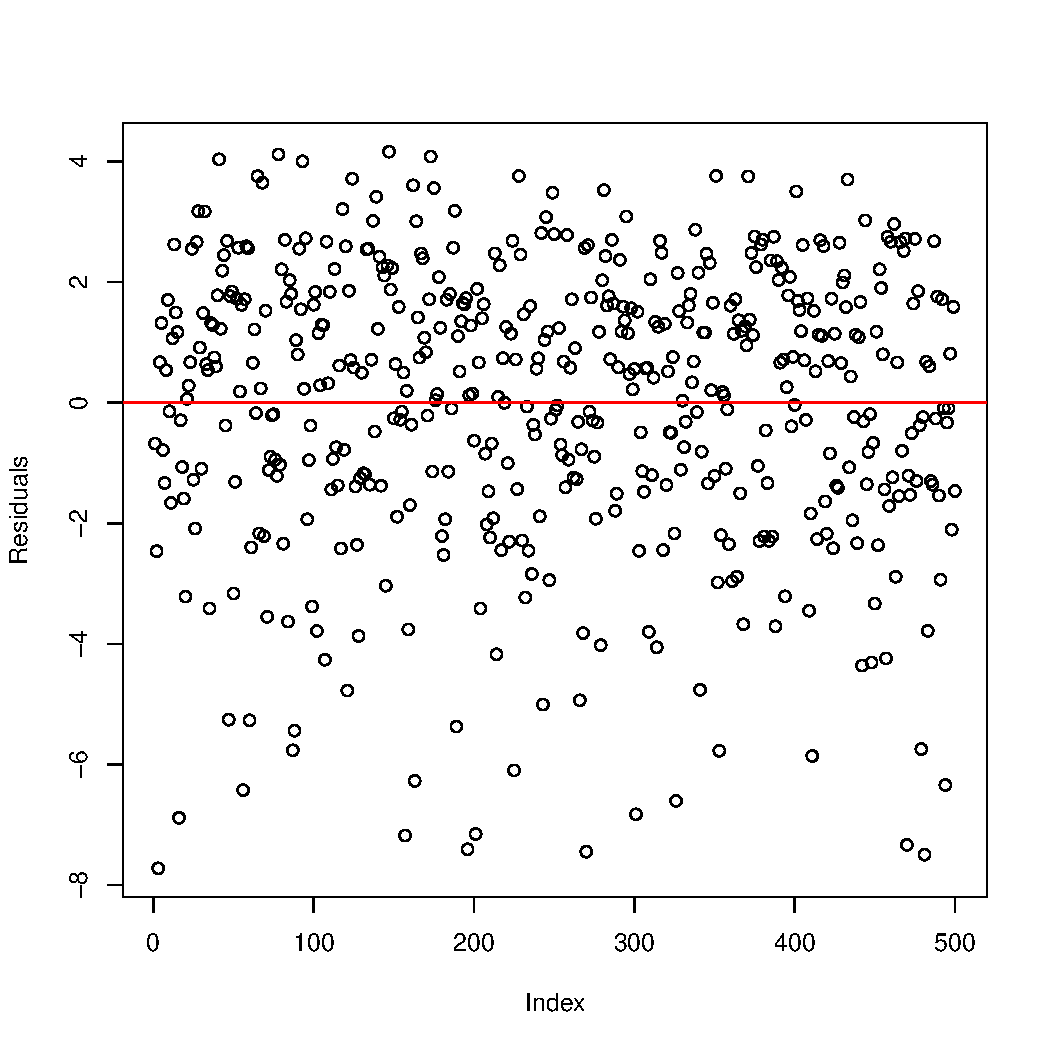
\includegraphics[width=4in]{../15_Diagnostics/siminresid.pdf}%this was not dynamic
          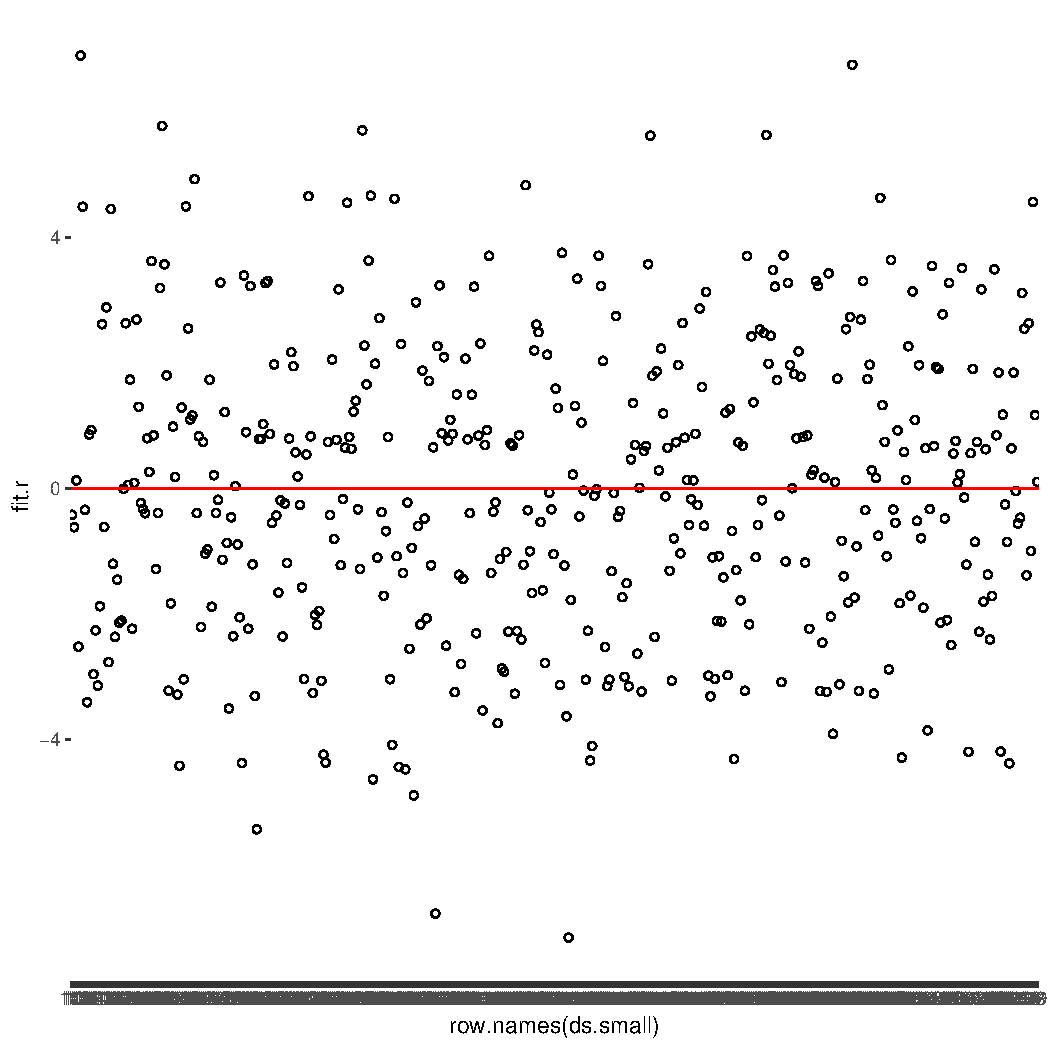
\includegraphics[width=4in]{../15_Diagnostics/multinresid.pdf}%filename
        \caption{Index Plot of Residuals: Multiple Regression \label{fig:siminresid}}
\end{figure}        

%Above graphic is not generated by R chunks. -- this may be fixed

Next, we can sort the residuals and find the case with the largest absolute value and examine that case.  

% largest residuals 
\begin{knitrout}
\definecolor{shadecolor}{rgb}{0.969, 0.969, 0.969}\color{fgcolor}\begin{kframe}
\begin{alltt}
\hlcom{#  Sort the residuals}
\hlstd{output.1} \hlkwb{<-} \hlkwd{sort}\hlstd{(ols1}\hlopt{$}\hlstd{residuals)}  \hlcom{# smallest first}
\hlstd{output.2} \hlkwb{<-} \hlkwd{sort}\hlstd{(ols1}\hlopt{$}\hlstd{residuals,} \hlkwc{decreasing} \hlstd{=} \hlnum{TRUE}\hlstd{)} \hlcom{# largest first}

\hlcom{#  The head function return the top results, the argument 1 returns 1 variable only}
\hlkwd{head}\hlstd{(output.1,} \hlnum{1}\hlstd{)} \hlcom{# smallest residual absolute value}
\end{alltt}
\begin{verbatim}
##       298 
## -7.161695
\end{verbatim}
\begin{alltt}
\hlkwd{head}\hlstd{(output.2,} \hlnum{1}\hlstd{)} \hlcom{# largest residual absolute value}
\end{alltt}
\begin{verbatim}
##       94 
## 6.898077
\end{verbatim}
\end{kframe}
\end{knitrout}

Then, we can examine the $X$ and $Y$ values of those cases on key variables. Here we examine the values across all independent variables in the model.  

\begin{knitrout}
\definecolor{shadecolor}{rgb}{0.969, 0.969, 0.969}\color{fgcolor}\begin{kframe}
\begin{alltt}
\hlstd{ds.small[}\hlkwd{c}\hlstd{(}\hlnum{298}\hlstd{,}\hlnum{94}\hlstd{),}\hlkwd{c}\hlstd{(}\hlstr{"age"}\hlstd{,}\hlstr{"education"}\hlstd{,}\hlstr{"income"}\hlstd{,}\hlstr{"ideol"}\hlstd{,}\hlstr{"glbcc_risk"}\hlstd{)]} \hlcom{# [c(row numbers),c(column numbers)]}
\end{alltt}
\begin{verbatim}
## # A tibble: 2 x 5
##     age education income ideol glbcc_risk
##   <int>     <int>  <dbl> <int>      <int>
## 1    69         6 100000     2          2
## 2    55         7  94000     7         10
\end{verbatim}
\end{kframe}
\end{knitrout}

By examining the case of 298, we can see that this is outlier because the observed values of $Y$ are far from what would be expected, given the values of $X$. A wealthy older liberal would most likely rate climate change as riskier than a 2. In case 94, a strong conservaitive rates climate change risk at the lowest possible value.  This observation, while not consistent with the estimated relationship between ideology and environmental concern, is certainly not implausible.  But the unusual appearance of a case with a strong conservative leaning, and high risk of cliamte change results in a large residual.

What we really want to know is: does any particular case substantially change the regression results? If a case  substantively change the results than it is said to have influence. Individual cases can be outliers, but still be influential.  Note that DFBETAS are \textbf{case statistics}, therefore a DFBETA value will be calculated for each variable for each case.   

\subsubsection{DFBETAS} 
DFBETAS measure the influence of case $i$ on the $j$ estimated coefficients. Specifically, it asks by how many standard errors does $B_j$ change when case $i$ is removed DFBETAS are expressed as:
\begin{equation}
  \label{eq:dfbeta}
  \text{DFBETAS}_{ij} = \frac{B_{j(-i)}-B_j}{SE(B_j)}
\end{equation}
Note that if DFBETAS $ > 0$, then case $i$ pulls $B_j$ \textit{up}, and  if DFBETAS $ < 0$, then case $i$ pulls $B_j$ \textit{down}.  In general, if $|\text{DFBETAS}_{ij}| > \frac{2}{\sqrt{n}}$ then these cases warrant further examination. Note that this approach gets the top 5\% of influential cases, given the sample size. For both simple (bi-variate) and  multiple regression models the DFBETA cut-offs can be calculated in \texttt{R}.  
\begin{knitrout}
\definecolor{shadecolor}{rgb}{0.969, 0.969, 0.969}\color{fgcolor}\begin{kframe}
\begin{alltt}
\hlstd{df} \hlkwb{<-} \hlnum{2}\hlopt{/}\hlkwd{sqrt}\hlstd{(}\hlnum{500}\hlstd{)}
\hlstd{df}
\end{alltt}
\begin{verbatim}
## [1] 0.08944272
\end{verbatim}
\end{kframe}
\end{knitrout}
\noindent In this case, if $|\text{DFBETAS}| > 0.0894427$ then they can be examined for  possible influence. Note, however, than in large datasets this may prove to be difficult,  so you should examine the largest DFBETAS first. In our example, we will look only at the largest 5 DFBETAS.

To calculate the DFBETAS we use the \texttt{dfbetas} function. Then we examine the DFBETA values for the first five rows of our data. 
\begin{knitrout}
\definecolor{shadecolor}{rgb}{0.969, 0.969, 0.969}\color{fgcolor}\begin{kframe}
\begin{alltt}
\hlstd{df.ols1} \hlkwb{<-} \hlkwd{dfbetas}\hlstd{(ols1)}
\hlstd{df.ols1[}\hlnum{1}\hlopt{:}\hlnum{5}\hlstd{,]}
\end{alltt}
\begin{verbatim}
##    (Intercept)          age   education      income        ideol
## 1 -0.004396485  0.005554545  0.01043817 -0.01548697 -0.005616679
## 2  0.046302381 -0.007569305 -0.02671961 -0.01401653 -0.042323468
## 3 -0.002896270  0.018301623 -0.01946054  0.02534233 -0.023111519
## 4 -0.072106074  0.060263914  0.02966501  0.01243482  0.015464937
## 5 -0.057608817 -0.005345142 -0.04948456  0.06456577  0.134103149
\end{verbatim}
\end{kframe}
\end{knitrout}
We can then plot the DFBETAS for each of the IVs in our  regression models, and create lines for $\pm 0.089$.  Figure \ref{fig:dfbetas} shows the DFBETAS for each variable in the multiple regression model.   

\begin{knitrout}
\definecolor{shadecolor}{rgb}{0.969, 0.969, 0.969}\color{fgcolor}\begin{kframe}
\begin{alltt}
\hlkwd{melt}\hlstd{(dfb.ols1,} \hlkwc{varnames} \hlstd{=} \hlkwd{c}\hlstd{(}\hlstr{"index"}\hlstd{,} \hlstr{"variable"}\hlstd{))} \hlopt
  \hlkwd{ggplot}\hlstd{(}\hlkwd{aes}\hlstd{(index, value))} \hlopt{+}
  \hlkwd{geom_point}\hlstd{()} \hlopt{+}
  \hlkwd{geom_hline}\hlstd{(}\hlkwc{yintercept} \hlstd{= df)} \hlopt{+}
  \hlkwd{geom_hline}\hlstd{(}\hlkwc{yintercept} \hlstd{=} \hlopt{-}\hlstd{df)} \hlopt{+}
  \hlkwd{facet_wrap}\hlstd{(}\hlopt{~} \hlstd{variable,} \hlkwc{scales} \hlstd{=} \hlstr{"free"}\hlstd{)}
\end{alltt}


{\ttfamily\noindent\bfseries\color{errorcolor}{\#\# Error in melt(dfb.ols1, varnames = c("{}index"{}, "{}variable"{})): object 'dfb.ols1' not found}}\begin{alltt}
\hlkwd{dev.off}\hlstd{()}
\end{alltt}
\end{kframe}
\end{knitrout}

\begin{figure}
        \centering
        \includegraphics[width=4in]{../15_Diagnostics/dfbetas.pdf}%filename
        \caption{Index Plot of DFBETAS: Multiple  Regression \label{fig:dfbetas}}
\end{figure}        

As can be seen, several cases seem to exceed the $0.089$ cut-off. Next we find the case with the highest absolute DFBETA value, and examine the $X$ and $Y$ values for that case. 
\begin{knitrout}
\definecolor{shadecolor}{rgb}{0.969, 0.969, 0.969}\color{fgcolor}\begin{kframe}
\begin{alltt}
\hlcom{###################}
\hlcom{#  Return Absolute Value dfbeta}
\hlkwd{names}\hlstd{(df.ols1)} \hlkwb{<-} \hlkwd{row.names}\hlstd{(ds.small)}
\hlstd{df.ols1[}\hlkwd{abs}\hlstd{(df.ols1)} \hlopt{==} \hlkwd{max}\hlstd{(}\hlkwd{abs}\hlstd{(df.ols1))]}
\end{alltt}
\begin{verbatim}
##      <NA> 
## 0.4112137
\end{verbatim}
\begin{alltt}
\hlcom{# a observation name may not be returned - let's figure out the observation}

\hlcom{#  convert df.osl1 from matrix to dataframe }
\hlkwd{class}\hlstd{(df.ols1)}
\end{alltt}
\begin{verbatim}
## [1] "matrix"
\end{verbatim}
\begin{alltt}
\hlstd{df2.ols1} \hlkwb{<-} \hlkwd{as.data.frame}\hlstd{(df.ols1)}

\hlcom{#  add an id variable}
\hlstd{df2.ols1}\hlopt{$}\hlstd{id} \hlkwb{<-} \hlnum{1}\hlopt{:}\hlnum{450} \hlcom{#  generate a new observation number}

\hlcom{#  head function returns one value, based on ,1}
\hlcom{#  syntax - head(data_set[with(data_set, order(+/-variable)), ], 1)}

\hlcom{#  Ideology}
\hlkwd{head}\hlstd{(df2.ols1[}\hlkwd{with}\hlstd{(df2.ols1,} \hlkwd{order}\hlstd{(}\hlopt{-}\hlstd{ideol)), ],} \hlnum{1}\hlstd{)} \hlcom{# order declining}
\end{alltt}
\begin{verbatim}
##      (Intercept)        age   education      income     ideol  id
## 298 -0.001083869 -0.1276632 -0.04252348 -0.07591519 0.2438799 298
\end{verbatim}
\begin{alltt}
\hlkwd{head}\hlstd{(df2.ols1[}\hlkwd{with}\hlstd{(df2.ols1,} \hlkwd{order}\hlstd{(}\hlopt{+}\hlstd{ideol)), ],} \hlnum{1}\hlstd{)} \hlcom{# order increasing}
\end{alltt}
\begin{verbatim}
##     (Intercept)       age   education     income       ideol  id
## 131  -0.0477082 0.1279219 -0.03641922 0.04291471 -0.09833372 131
\end{verbatim}
\begin{alltt}
\hlcom{#  Income}
\hlkwd{head}\hlstd{(df2.ols1[}\hlkwd{with}\hlstd{(df2.ols1,} \hlkwd{order}\hlstd{(}\hlopt{-}\hlstd{income)), ],} \hlnum{1}\hlstd{)} \hlcom{# order declining}
\end{alltt}
\begin{verbatim}
##     (Intercept)         age    education    income       ideol  id
## 445 -0.05137992 -0.01514244 -0.009938873 0.4112137 -0.03873292 445
\end{verbatim}
\begin{alltt}
\hlkwd{head}\hlstd{(df2.ols1[}\hlkwd{with}\hlstd{(df2.ols1,} \hlkwd{order}\hlstd{(}\hlopt{+}\hlstd{income)), ],} \hlnum{1}\hlstd{)} \hlcom{# order increasing}
\end{alltt}
\begin{verbatim}
##     (Intercept)         age  education     income      ideol  id
## 254  0.06766781 -0.06611698 0.08166577 -0.4001515 0.04501527 254
\end{verbatim}
\begin{alltt}
\hlcom{#  Age}
\hlkwd{head}\hlstd{(df2.ols1[}\hlkwd{with}\hlstd{(df2.ols1,} \hlkwd{order}\hlstd{(}\hlopt{-}\hlstd{age)), ],} \hlnum{1}\hlstd{)} \hlcom{# order declining}
\end{alltt}
\begin{verbatim}
##    (Intercept)       age  education      income     ideol id
## 78  -0.2146905 0.1786665 0.04131316 -0.01755352 0.1390403 78
\end{verbatim}
\begin{alltt}
\hlkwd{head}\hlstd{(df2.ols1[}\hlkwd{with}\hlstd{(df2.ols1,} \hlkwd{order}\hlstd{(}\hlopt{+}\hlstd{age)), ],} \hlnum{1}\hlstd{)} \hlcom{# order increasing}
\end{alltt}
\begin{verbatim}
##     (Intercept)        age  education     income     ideol  id
## 420    0.183455 -0.2193257 -0.1906404 0.02477437 0.1832784 420
\end{verbatim}
\begin{alltt}
\hlcom{#  Education - we find the amount - ID 308 for edu}
\hlkwd{head}\hlstd{(df2.ols1[}\hlkwd{with}\hlstd{(df2.ols1,} \hlkwd{order}\hlstd{(}\hlopt{-}\hlstd{education)), ],} \hlnum{1}\hlstd{)} \hlcom{# order declining}
\end{alltt}
\begin{verbatim}
##     (Intercept)        age education      income      ideol  id
## 308  -0.1751724 0.06071469 0.1813973 -0.05557382 0.09717012 308
\end{verbatim}
\begin{alltt}
\hlkwd{head}\hlstd{(df2.ols1[}\hlkwd{with}\hlstd{(df2.ols1,} \hlkwd{order}\hlstd{(}\hlopt{+}\hlstd{education)), ],} \hlnum{1}\hlstd{)} \hlcom{# order increasing}
\end{alltt}
\begin{verbatim}
##    (Intercept)       age  education      income        ideol id
## 95  0.05091437 0.1062966 -0.2033285 -0.02741242 -0.005880984 95
\end{verbatim}
\begin{alltt}
\hlcom{#  View the output}
\hlstd{df.ols1[}\hlkwd{abs}\hlstd{(df.ols1)} \hlopt{==} \hlkwd{max}\hlstd{(}\hlkwd{abs}\hlstd{(df.ols1))]}
\end{alltt}
\begin{verbatim}
##      <NA> 
## 0.4112137
\end{verbatim}
\begin{alltt}
\hlstd{df.ols1[}\hlkwd{c}\hlstd{(}\hlnum{308}\hlstd{),]} \hlcom{# dfbeta number is observation 131 - education}
\end{alltt}
\begin{verbatim}
## (Intercept)         age   education      income       ideol 
## -0.17517243  0.06071469  0.18139726 -0.05557382  0.09717012
\end{verbatim}
\begin{alltt}
\hlstd{ds.small[}\hlkwd{c}\hlstd{(}\hlnum{308}\hlstd{),} \hlkwd{c}\hlstd{(}\hlstr{"age"}\hlstd{,} \hlstr{"education"}\hlstd{,} \hlstr{"income"}\hlstd{,} \hlstr{"ideol"}\hlstd{,} \hlstr{"glbcc_risk"}\hlstd{)]}
\end{alltt}
\begin{verbatim}
## # A tibble: 1 x 5
##     age education income ideol glbcc_risk
##   <int>     <int>  <dbl> <int>      <int>
## 1    51         2  81000     3          4
\end{verbatim}
\end{kframe}
\end{knitrout}

Note that this ``severe outlier" is indeed an interesting case -- a 51 year old with a high school diploma, relatively high income, who is slightly liberal and perceivs low risk for climate change. But this outlier is not implausible, and therefore we can be reassured that -- even in this most extreme case -- we do not have problematic outliers.

So, having explored the residuals from our model, we found a number of outliers, some with  significant influence on our model results. In inspection of the most extreme outlier gave us no cause to worry that the observations were inappropriately distorting our model results. But what should you do if you find puzzling, implausible observations that may  influence your model?

First, as always, evaluate your theory. Is it possible that the case represented a class of observations that behave systematically differently than the other cases? This is of particular concern if you have a cluster of cases, all determined to be outliers, that have similar properties. You may need to modify your theory to account for this subgroup. One such example can be found in the study of American politics, wherein the Southern states routinely appeared to behave differently than others. Most careful efforts to model state (and individual) political behavior account for the unique aspects of southern politics, in ways ranging from the addition of dummy variables to interaction terms in regression models.

How would you determine whether the model (and theory) should be revised? Look closely at the deviant cases -- what can you learn from them? Try experiments by running the models with controls -- dummies and interaction terms. What effects do you observe? If your results suggest theoretical revisions, you will need to collect new data to test your new hypotheses. Remember: In empirical studies, you need to keep your discoveries distinct from your hypothesis tests.

As a last resort, if you have troubling outliers for which you cannot account in theory, you might decide omit those observations from your model and re-run your analyses. We do not recommend this course of action, because it can  appear to be a case of ``jiggering the data" to get the results you want. 

\subsection{Multicollinearity} 

Multicollinearity is the correlation of the IVs in the model. Note that if any $X_i$ is a linear combination of other $X$'s in the model, $B_i$ cannot be estimated. As discussed previously, the partial regression coefficient strips both the $X$'s and $Y$ of the overlapping covariation by regressing one $X$ variable on all other $X$ variables: 
\begin{align*}
  E_{X_{i}|X_{j}} &= X_i - \hat{X}_i \\
  \hat{X}_i &= A + BX_j 
\end{align*}
If an X is perfectly predicted by the other $X$'s, then:
\begin{center}
  $E_{X_{i}|X_{j}}=0$ 
  
  and 
  
  $R^2_k=1$
\end{center}
\noindent where $R^2_k$ is the $R^2$ obtained from regressing all
$X_k$ on all other $X$'s. 

We rarely find perfect multicollinearity in practice, but high multicollinearity results in loss of statistical resolution. Such as:  
\begin{itemize}
\item Large standard errors
\item Low $t$-stats, high $p$-values
  \begin{itemize}
\item This erodes the resolution of our hypothesis tests
  \end{itemize}
\item Enormous sensitivity to small changes in:
  \begin{itemize}
\item Data
\item Model specification
  \end{itemize}
  \end{itemize}

You should always check the correlations between the IVs during the model building process. This is a way to quickly identify possible multicollinearity issues.
\begin{knitrout}
\definecolor{shadecolor}{rgb}{0.969, 0.969, 0.969}\color{fgcolor}\begin{kframe}
\begin{alltt}
\hlstd{ds} \hlopt
  \hlkwd{select}\hlstd{(age, education, income, ideol)} \hlopt
  \hlkwd{na.omit}\hlstd{()} \hlopt
  \hlkwd{data.frame}\hlstd{()} \hlopt
  \hlkwd{cor}\hlstd{()}
\end{alltt}
\begin{verbatim}
##                   age   education      income       ideol
## age        1.00000000 -0.06370223 -0.11853753  0.08535126
## education -0.06370223  1.00000000  0.30129917 -0.13770584
## income    -0.11853753  0.30129917  1.00000000  0.04147114
## ideol      0.08535126 -0.13770584  0.04147114  1.00000000
\end{verbatim}
\end{kframe}
\end{knitrout}
\noindent There do not appear to be any variables that are so highly correlated that it would result in problems with multicolinearity. 

We will discuss two more formal ways to check for multicollinearity. First, is the  \textbf{Variance Inflation Factor} (VIF), and the second is \textbf{tolerance}. The VIF is the  degree to which the variance of other coefficients is increased due to the inclusion of the specified variable. It is expressed as: 

\begin{equation}
  \label{eq:vif}
  \text{VIF} = \frac{1}{1-R^2_k}
\end{equation}

\noindent Note that as $R^2_k$ increases the variance of $X_k$ increases. A general rule of thumb is that $\text{VIF} > 5$ is problematic. 

Another, and related, way to measure multicollinearity is tolerance. The tolerance of any $X$, $X_k$, is the proportion of its variance not shared with the other $X$'s. 
\begin{equation}
  \label{eq:tolerance}
  \text{tolerance} = 1-R^2_k 
\end{equation}

\noindent Note that this is mathematically equivalent to $\frac{1}{VIF}$. The rule of thumb for acceptable tolerance is partly a function of $n$-size:

%\begin{SingleSpace} 
 
\begin{itemize}
\item If $n < 50$, tolerance should exceed $0.7$
\item If $n < 300$, tolerance should exceed $0.5$
\item If $n < 600$, tolerance should exceed $0.3$
\item If $n < 1000$, tolerance should exceed $0.1$
\end{itemize}

%\end{SingleSpace}

%But: watch for effects on other IVs

Both VIF and tolerance can be calculated in \texttt{R}. 
\begin{knitrout}
\definecolor{shadecolor}{rgb}{0.969, 0.969, 0.969}\color{fgcolor}\begin{kframe}
\begin{alltt}
\hlkwd{library}\hlstd{(car)}
\hlkwd{vif}\hlstd{(ols1)}
\end{alltt}
\begin{verbatim}
##       age education    income     ideol 
##  1.024094  1.098383  1.101733  1.009105
\end{verbatim}
\begin{alltt}
\hlnum{1}\hlopt{/}\hlkwd{vif}\hlstd{(ols1)}
\end{alltt}
\begin{verbatim}
##       age education    income     ideol 
## 0.9764731 0.9104295 0.9076611 0.9909775
\end{verbatim}
\end{kframe}
\end{knitrout}
\noindent Note that, for our example model, we are well within acceptable limits on both VIF and tolerance. 

%% what to do 
If multicollinearity is suspected, what can you do? One option is to drop one of the highly co-linear variables. However, this may result in model mis-specification. As with other modeling considerations, you must use theory as a guide. A second option would be to add new data, thereby lessening the threat posed by multicolinearity. A third option would be to obtain data from specialized  samples that maximize independent variation in the collinear variables (e.g., elite samples may disentangle the effects of income, education, and other SES-related variables). 

Yet another strategy involves reconsidering why your data are so highly  correlated. It may be that your measures are in fact different ``indicators" of the same underlying theoretical concept. This can happen, for example, when you measure sets of attitudes that are all influenced by a more general attitude or belief system. In such a case, data scaling is a promising option. This can be accomplished by building an additive scale, or using various scaling options in $R$. Another approach would be to use techniques such as factor analysis to tease out the underlying (or ``latent") variables represented by your indicator variables. Indeed, the combination of factor analysis and regression modeling is an important and widely used approach, referred to as structural equation modeling (SEM).  But that is a topic for another book and another course.

\section{Summary}
In this chapter we have described how you can approach the diagnostic stage for OLS multiple regression analysis. We described the key threats to the necessary assumptions of OLS, and listed them and their effects in Table \ref{tab:ass}. But we also noted that diagnostics are more of an art than a simple recipe. In this business you will learn as you go, both in the analysis of a particular model (or set of models) and in the development of  your own approach and procedures. We wish you well, Grasshopper!
\end{document}
